\documentclass[12pt,a4paper]{report}

\newenvironment{tightcenter}{%
  \setlength\topsep{0pt}
  \setlength\parskip{0pt}
  \begin{center}
}{%
  \end{center}
}

%%% User packages
\usepackage{wrapfig}
\usepackage{afterpage}
\usepackage{parskip} % Disable US-type paragraph
\usepackage[hyphens]{url}
\usepackage{titlesec}
\usepackage{xfrac}
\usepackage[usenames,dvipsnames,svgnames,table]{xcolor}
\usepackage{lastpage}
\usepackage{tocloft}
\usepackage{float}
\usepackage{fancybox, graphicx}
\usepackage[footnote,draft,english,silent,nomargin]{fixme}

%%% Tag specific
%\usepackage{tabularx} % Table
\usepackage{booktabs} % Nice tabelsMost critical path with backtracing
\usepackage{fancyhdr} % header & footer

%%% Layout related
\usepackage[left=2.5cm,right=2.5cm,top=2.5cm,bottom=2.5cm]{geometry} % Page margin

%%% Reference related
\usepackage[backend=bibtex]{biblatex}

%%% TOC
\setcounter{tocdepth}{1}

\bibliography{Kilder/kilder.bib}
%\PassOptionsToPackage{hyphens}{url}

%%% Font related
\usepackage{kmath,kerkis}
\usepackage{microtype}
\usepackage{mathptmx}
\usepackage[T1]{fontenc} 
\usepackage[utf8]{inputenc} %%\usepackage[utf8x]{inputenc}
\usepackage{amsfonts} % Math 
\usepackage[font=scriptsize]{caption} %small caption text

%%% Codeinput related
\usepackage[ruled]{algorithm2e}
\usepackage{listings} % Så man kan indsætte pæn kode, spørg Anders for hjælp
\usepackage{color}
\lstdefinelanguage{CSharp}
{
sensitive=false,
morekeywords=[1]{
abstract, as, base, break, case,
catch, checked, class, const, continue,
default, delegate, do, else, enum,
event, explicit, extern, false,
finally, fixed, for, foreach, goto, if,
implicit, in, interface, internal, is,
lock, namespace, new, null, operator,
out, override, params, private, foreach
protected, Task, Tasks, List, public, readonly, ref,
return, sealed, sizeof, var, stackalloc,
static, struct, switch, this, throw,
true, try, typeof, unchecked, TimeSpan, unsafe,
using, virtual, volatile, while, bool,
byte, char, decimal, double, float,
int, lock, object, sbyte, short, string,
uint, ulong, ushort, void, get, set},
morecomment=[l]{//},
morecomment=[s]{/*}{*/},
morecomment=[l][keywordstyle4]{\#},
morestring=[b]",
morestring=[b]',
}
\lstset{
backgroundcolor=\color[rgb]{0.95, 0.95, 0.95},
tabsize=2,
rulecolor=,
basicstyle=\scriptsize,
upquote=true,
aboveskip={1.5\baselineskip},
columns=fixed,
showstringspaces=false,
extendedchars=true,
breaklines=true,
frame=single,
showtabs=false,
showspaces=false,
showstringspaces=false,
identifierstyle=\ttfamily,
keywordstyle=\color[rgb]{1.0,0,0},
keywordstyle=[1]\color[rgb]{0,0,0.75},
keywordstyle=[2]\color[rgb]{0.5,0.0,0.0},
keywordstyle=[3]\color[rgb]{0.127,0.427,0.514},
keywordstyle=[4]\color[rgb]{0.4,0.4,0.4},
commentstyle=\color[rgb]{0.133,0.545,0.133},
stringstyle=\color[rgb]{0.639,0.082,0.082},
} % Dokument der tilader at bruge C# farvestil i kode indsættelse
\lstset{language=[Sharp]C} 
\lstdefinestyle{csharp2}{language=[Sharp]C, frame=lr, rulecolor=\color{blue!80!black}}

\makeatletter
\renewcommand\part{%
    \if@openright
        \cleardoublepage
    \else
        \clearpage
    \fi
    \thispagestyle{empty}%
    \if@twocolumn
        \onecolumn
        \@tempswatrue
    \else
        \@tempswafalse
    \fi
    \null\vfil
    \secdef\@part\@spart}
\makeatother

\AtBeginDocument{\addtocontents{toc}{\protect\thispagestyle{empty}}} 

\titleformat{\chapter}{\normalfont\huge\bfseries}{ \thechapter.}{20pt}{\huge}
\setcounter{section}{0}
\pagestyle{fancy}
\fancypagestyle{arabic}
{
    \fancyhf{}
    \setlength{\headheight}{15pt}
}



%\titleformat{\chapter}[display]   
%{\normalfont\huge\bfseries}{\chaptertitlename\ \thechapter}{20pt}{\Huge}   
\titlespacing*{\chapter}{-10pt}{-20pt}{10pt}

\renewcommand{\chaptermark}[1]{ \markboth{#1}{} }
\fancypagestyle{chp}{
  \fancyhf{}
    \lhead{\MakeUppercase{\leftmark}}
  \rhead{\rightmark}%\colorbox{black}{\color{white}{\rightmark}}}
  \cfoot{\thepage\ of \pageref{LastPage}}
}
\fancypagestyle{plain}{
    %\fancyhf{}
  \cfoot{\thepage\ of \pageref{LastPage}}
}

\newcommand*{\blankpage}{%
\vspace*{\fill}
\centering \textit{This page intentionally left (almost) blank.}
\vspace{\fill}}

\pagestyle{fancy}

\title{
    \vspace*{-3cm}
    \fontsize{50}{48} \textbf{Titel TBA}\\
    \fontsize{20}{48}\emph{A software analysis and -implementation}
}
\author{
    \noindent\makebox[\textwidth]{%
    
\includegraphics[width=1.2\textwidth]{Grafik/ForsideUmodificeret.png}\hspace*{0.5cm}}\\
    \emph{Mathias Vestergaard Rasmussen}\\
    \emph{Christoffer Carlé Christensen}\\
    \emph{Kasper Østergaard Helsted}\\
    \emph{Anders Lykke Matthiassen}\\
    \emph{Christian Stephansen}\\
    \emph{Gideon Blegmand}
}

\date{19 - 12 - 2014}


\definecolor{codecomment}{HTML}{383838}

\lstset{language=C,
    basicstyle=\ttfamily\scriptsize,
    keywordstyle=\color{Blue}\ttfamily,
    otherkeywords={WIDTH},
    keywords=[2]{__shared__},
    keywordstyle=[2]\color{orange}\ttfamily,
    stringstyle=\color{red}\ttfamily,
    commentstyle=\color{codecomment}\ttfamily,
    breaklines=true,
    numbers=left,
}

\usepackage[bookmarks]{hyperref}
\hypersetup{pdftex, hidelinks=true}
\usepackage{hypcap}
\DeclareUnicodeCharacter{00A0}{~}

\usepackage{cleveref}

\begin{document}
    \addtocontents{toc}{\protect\thispagestyle{empty}}
    \maketitle
    \afterpage{\blankpage}
        \thispagestyle{empty}
    %\pagenumbering{gobble}
    \clearpage
    %Titlepage 
    \thispagestyle{empty}
\begin{titlepage}
    \setlength{\textwidth}{15cm}
    \noindent
    \begin{nopagebreak}
        {\samepage 
            \begin{tabular}{lr}
                \parbox{0.5\textwidth}{\raisebox{11mm}
                    {
\includegraphics[height=2.2cm]{Grafik/aauLogoDa2}}
                } &
                \parbox{0.5\textwidth}{
                    \small
                    \begin{tabular}{l}
                        {\sf\small \textbf{Department of Computer Science }}\\
                        {\sf\small CASSIOPEIA} \\
                        {\sf\small Selma Lagerløfs Vej 300} \\
                        {\sf\small DK-9220 Aalborg Ø.} \\
                    \end{tabular}
                }
            \end{tabular}
            
            \noindent
            \begin{tabular}{cc}
                \parbox{7cm}{
                    \begin{description}
            
                        \item {\bf Title:} 
            
                            \textbf{Meal Planner}\\
                        \item {\bf Project Period:}\\
                            Autumn Semester 2014\\
                            \hspace{4cm}
                        \item {\bf Project Group:}\\
                            SW3-ds301e14\\
                            \hspace{4cm}
                        \item {\bf Participants:}\\
                            Mathias Vestergaard Rasmussen\\
                            Christoffer Carlé Christensen\\
                            Kasper Østergaard Helsted\\
                            Anders Lykke Matthiassen\\
                            Christian Stephansen\\
                            Gideon Blegmand\\
                            \hspace{2cm}
                        \item {\bf Supervisor:}\\
                            Rudra Pratap Deb Nath\\

                        \item {\bf Copies:}\\ 9\\
                        \item {\bf Page Numbers:}\\ 117\\
                        \item {\bf Appendix:}\\ Page 92-117\\
                        \item {\bf Date of Completion:}\\ 19-12-2014\\
                    \end{description}
                    \vfill
                } &
                \parbox{7cm}{
                    \vspace{.15cm}
                    \hfill 
                    \begin{tabular}{l}
                        {\bf Abstract:}\bigskip \\
                        \fbox{
                            \parbox{6.5cm}{\smallskip
                                {\vfill{\small %\section* {Synopsis}

                                \smallskip}}
                            }
                        }
                    \end{tabular}
                }
            \end{tabular}
        }\\
        \\
        \noindent{\footnotesize\emph{The contents of this report is freely accessible, but publication (with referencing) may only happen under agreement with the authors.}}
    \end{nopagebreak}
\end{titlepage}

    \afterpage{\blankpage}
        \thispagestyle{empty}
    %\pagenumbering{gobble}
    \clearpage
    %\pagenumbering{roman}
    \chapter*{Preface} \label{PrefaceLabel}

This report is a result of the hard work of Anders Lykke Matthiassen, Christian Stephansen, Christoffer Carlé Christensen, Gideon Blegmand, Kasper Østergaard Helsted, and Mathias Vestergaard Rasmussen.

The intellectual property rights of this report and all of its contents belong to the members of the project. All material gathered from third party resources will be referred to according to the IEEE standard.

The source code for the software solution of the project, is open source, under the Beerware license. The code is freely available at https://github.com/Helstedxd/FoodPlanner-Project.

The colours for this program, were chosen by using an online tool called Paletton \cite{paletton}, which suggests a colour theme based on the colours the user choose. The figures used in the report, have been created using Visio and Inkscape, unless stated otherwise.

The authors would like to thank participants of the Usability test for their time and constructive critique, as well as the informants for the interviews and user stories, for their cooperation. The report makers would also like to thank Rudra Pratap Deb Nath for his help and constructive criticism throughout the project process.

        \thispagestyle{empty}
    %\renewcommand*\contentsname{Indholdsfortegnelse}
    \newpage
        {\pagestyle{empty}
    \tableofcontents
    \cleardoublepage}
    \pagenumbering{arabic}
    \clearpage
    \setcounter{page}{1}
    \pagestyle{plain}
    
    \part{Introduction}
	\section{Waterfall method}

In the group it was chosen to use the waterfall method for the project. In this section the reason for this choice and a general description of the waterfall method will be given, with focus on the groups use of the method. The waterfall method means that you start in one end of the product and finishes in the other, without going back to a part when you have finished it, where as the iterative approach focuses on going in a circle, and doing the project many times, expanding the product and report each time. The strengths of the waterfall method, focuses on the ease of setting dealines throughput the project, knowing when a part is finished, it will not need to be revisited. The weaknesses though is that if the information the project is based on changes or have more information added, as more analysis would be needed. 

The waterfall method includes 5 steps:

\begin{itemize}
	\item Analysis
	\item Design
	\item Implementation
	\item System test
	\item In operation
\end{itemize}

\textbf{The analysis part} of the waterfall method focus on getting to know your target audience. This is the part of the report that is called problem analysis, which includes the sources of information that was found. In this part of the project, the specific goal of the product was defined, and the part ended out with the requirement specifications. It was also in this section that the interviews where conducted.

\textbf{The design part} of the waterfall method is focused on the design of the software. In the project, the design part focused on the principles learned in the course "Design and Evaluation of User Interfaces". This includes things like a PACT analysis. At the end of the design part, the design specifications were found. The design also includes the principles learned in sytem development, so inn this part the class diagrams and such were also made.

\textbf{The implementation part} of the system, is the part in which the software is created. The design specification is used to make the design, and the needed functionality which was discovered in the analysis as being the requirement specifications is implemented in the product. The outcome of this was the system itself.

\textbf{The system test} is the fourth part of the waterfall method, in this part the system is tested to see if it works, and fulfills the requirements. The outcome of this part of the method is a test report, which are included in the report.\fxnote{Insert reference to where in the report, when this is known.}

\textbf{The system in operation} is the last part. When the system is public, and the outcome of this is a status of the operation. This part though is not implemented in this system, as the product the group makes will not be available for the public to use.

The reason that the waterfall method was chosen for this project, was that a lot of new information would not come throughout the project. Food waste is and will be a problem, and some sort of product is needed to change this. Therefore it seemed natural to gather all the information at first, and work out from that. The waterfall method lived up to the expectiations of the group, meaning that deadlines where kept so the project was on track all of the time.

    \part{Problem Analysis}
    	\section{Foodplan study}
\textit{Stop Spild Af Mad}\cite{madSpild_RapportAdfaerd} has conducted a study where eight informants had had to create and follow a weekly food-schedule.
Each participants had to create a foodplan and they could freely choose the different recipes with inspiration from cookbooks or the internet.

\subsection*{Planning}
The informants had some trouble with pulling them self together and getting started creating the foodplan, but they were happy to have it, once it was done. It could be beneficial for the person that were in charge of grocery-shopping, to be the one making the schedule, since the involvement of other members from the family could increase the time of making it.

\subsection*{Modules}
It was almost impossible for the informants to follow the schedule for a whole week, without having to reorganize or modify it. Most of the informants made small modules, that could be moved around depending on the family's situation. It was optimal with modules spanning two-three days. Varied meals was preferred, and not simply reheated meals.

\subsection*{grocery-shopping}
Seven out of the eight participants was shopping groceries almost every day. This was not seen as a nuisance, but after having planned grocery-shopping for a whole week, they experienced a big relief in their everyday life. This was expressed in terms of more personal freedom as a consequence of saving time and money. Planning ahead also decreased buying on impulse.
\fxnote{textbf might be a bad choice.. CHS tried using emphasize on Less gro... and subsubsec on Modules (subsubsec throws a warning because we have no subsec beforehand .. please evaluate, on which type we should use.}

\subsection{Reflection} \fxnote{This is some sort of conclusion/reflection for this section, but might need to be moved.}
The participant had trouble getting started creating a new food plan for the week. They also wanted a more realistic food-schedule instead of having to create it from cookbooks. Realistic in the sense that the plan should fit into their context. A solution to this problem might be solved by automating a lot of the tasks involved with having to come up with the different recipes and do the grocery shopping.
By having an application come up with suggested meals based on different aspects such as the:
\begin{itemize}
\item Food you already have
\item Food you like
\item Price
\item Stock of stores nearby
\end{itemize}
People could quickly create the schedule or maybe even have the application create it for them.
\section{FDB Report}
The following section examines a report published in 2011 by FDB called "Forbrugerne: Vi smider ikke mad ud"\cite{madSpild_FDB}.
\subsection{Method used in the report}
The report is an anthropological study of how food waste occurs and how it is experienced by the consumers. The study is based on qualitative data collected from six different households. These households are all different from one another e.g. they live in different geographical locations. Data is gathered from the participants by using observations e.g. watching participants shop or prepare food, semi-structured interviews and probing kits. The data is then used to examine the activity patterns and motivation of the participants.

\subsection{FDB report: What is food waste and how does it occur.}
The report discusses why food waste occurs and how the participants perceive it. There are some subjects that are interesting when learning about food waste. 

\subsubsection{What is food waste}
When the participants was asked how much food they threw out, they typically answered that they threw out as little as possible. There is a clear distinction between waste and non-waste being thrown out. It is acceptable to throw waste out, but not to do the same with non-waste. The waste and non-waste categories varies depending on cooked food products and uncooked food products. Cooked food is considered waste when larger parts, or leftovers of a meal that has not been served on a plate is thrown out. So when the food has been served on a plate it is acceptable to throw it out. Uncooked food is considered waste when the packaging is unopened. It is not considered waste when the uncooked fat or other food parts that are considered non-edible is thrown out.

\subsubsection{Cause of food waste} 
The reasons as to why food is thrown out varies depending on cooked and uncooked products. Uncooked products is thrown out because they are bought in so large quantities that the consumers were not able to eat it prior to expiry. Products that are considered non-edible such as cartilage or bad vegetables are also thrown out. Cooked food products are also likely to be thrown out. Cooked food products are thrown out because the participants prepared more than they could eat in one meal. If the participants estimated that there were enough leftovers to save them for later they would. But often the leftovers was stored in the fridge for 4 days only to be thrown out.

\subsubsection{Food waste barriers}
The participants might have the will to reduce food waste but there are some barriers that can impact the participants will in a negative way. The status \fxnote{status/value formulation} of the meal ingredients can be a barrier. Dinner is often based around the chosen kind of meat because it has more value. This means that all other ingredients on a plate only is supplementary. It is easier to throw away the supplements than the meat because of its status. Therefore supplements represents a larger part of the food waste in the homes. Making a large delicious and fresh meal is also a way to show appreciation towards guests or household members. This can also act as a barrier because it requires the food to be fresh and in large amounts. Another barrier is quantity discounts. It contradicts with the participants reasoning when they have to decide between buying what is the right economical, or what is right according to food waste. In the situation people often think of the economical aspects, and not on what they will do with the extra food. The participants also expressed a lack of overview of what products they had at home when they were out shopping. Sometimes they bought something that they already had, because they was not sure if they had it at home. This results in an overstocking of a product that is most likely to be thrown out. Another barrier was planning versus impulse and desire. Participants that shopped regularly, said that they sometimes changed their minds on what they wanted for dinner or that they wanted variation in their dinners. This spontaneity and need for variation could result in products being bought for one night and the leftovers being stored and in the end being thrown out. Participants that shopped frequently said that they wanted variation and therefore did not plan dinners for a whole week. This could result in a lack of overview and in the end more food waste. The expiration date can also affect the participants willingness to buy a product. The tolerance of when a product is not edible varies between participants, and when the product can give a smell or a visual sign of decay. The expiration date had less importance. The last barrier that is discussed is what is acceptable as food waste. Some of the barriers that has been mentioned is accepted in some degree by the participants. One of the participants talks about the acceptance of food waste when it comes from a child's plate. The participants says that it is to hard assess how much the child will eat and that it leads to food waste but it is a waste the participant will accept.
\section{How to avoid food waste}

According to The Danish Ministry of the Environment, one of the initiatives you can take against food waste, is to make recipes which incorporate the leftovers, or what is left in the refrigerator. By doing this food that might otherwise go bad, will be used instead of being thrown away. http://mindremadspild.dk/files/mindremadspild_idekatalog_150611.pdf

Another Initiative that can be taken according to The Danish Ministry of the Environment, is to sell quantity discount, with the option to recieve some of the groceries later. An example would be if 1 cucumber is sold for 10 DKK, while 2 is sold for 15, some people would choose to buy 2 cucumbers because of the quantity discount, even if they just needed 1 at the moment. With a "recieve later" option, you would be able to buy 2 cucumbers, but only recieve 1 at the moment. Then you would be able to come back to the store later to get the other cucumber when you needed it. An initiative like this have already been made by the English supermarket chain Tesco. The initiative is called "Buy One Get One Free Later", and is an initiative for fresh groceries like fruit and vegetables.

To give the consumer better information about when food is going bad is also an initiative that The Danish Ministry of Environment is recommending. By informing consumers of what "Best before", "Last day of sale" and so on means, would get the consumer to use the food more properly. Also by getting the consumer to rely more on smell, taste and looks, rather than just the date of production on the groceries, would lead to lesser food waste.

The Danish Ministry of the Environment, also reccomend getting discounts even thoug you don't buy in quantity. Being able to share an offer with another person would let the supermarkets get volumes bought, and the consumer would be able to only aquire the amount neccessairy.

Only using the gorecries neccessairy is also a way to achieve lesser food waste. Following Recipes will help with this if the recipes is specific. If for example the repicipe is for 4 persons, and 4 persons will be eating, if the recipe is correct food will not be wasted, and even if there are leftovers after the meal, using these as lunch for the next day, or eating the leftovers the day after, will achieve a lesser waste of food. http://www.brugmerespildmindre.dk/mindre-madspild


\section{Food waste}
Every year danish households throws away nearly 237.000 tons of food, that could have been eaten by people. This is estimated to be nearly 16 mio DKK. About 20 \% of a danish households foodbudget is wasted by throwing away food that could have been eaten, this means that if there was no food waste at all, 1 million people could be fed, this is nearly 1/5 of the danish people.

The people who throws away most food, are the people living alone. The average person living alone throws away 98.8 kg of food per year, where as a household with 5 people throws away 46.8 kg of food per person per year. It is mostly dairy products, vegetables and bread that gets thrown away, though in december a lot of meat is also thrown away, due to the fact that it is Christmas, where people eat more food.

Since 2007 the danish people have been purchasing 10 \% less food, a lot of this food used to end up in the trashcan as food waste. 54 \% of the danish people rarely or never uses the food from the night before for later eating, and 69 \% does not use leftovers for lunch the day after. Elderly people are better at using leftovers than younger people. \fxnote{references to bibliography, and/or maybe some graphs to show the numbers?}

20 \% of danish people does not make a grocery shopping list before going grocery shopping. 52 \% of people does not make a meal plan, 31 \% does sometimes and 17 \% does it often.

81 \% of danish people would use leftovers to avoid food waste, 50 percent would make a mealplan and make a grocery shopping list. 59 \% of the consumers believe that the danish food waste is their own fault.

\input{Analysis/StateOfTheArt.tex}

\chapter{PACT Analysis}
In this chapter, a pact analysis will be conducted in order to acquire a clearer view of how the main audience for the solution will behave. The information will be needed in order to find the requirements.
\section{People}
Everyone needs food, and many also have to buy and make it themselves. There are many ways to prepare a meal, and people have different preferences of what they eat and why. In this analysis the focus will be on the social, physical and psychological differences between people and on a description of their different motives and preferences. This description will be used to get an idea of who could benefit from a system, that would help them organize grocery shopping and preparing meals more efficiently.

\subsection{Physical differences}

People have different physical abilities. Some people have bad vision, some have bad hearing, and so on with a lot of different physical conditions, and taking this into considoration is an important aspect of a PACT analysis.

Looking at the ergonomically aspects of the application, is not necerrairy, since the ergonomics are decided by the company who creates the device that the application run on. Therefore ergonomics are not something that can be affected by the application.

\subsection{Psychological differences}

People vary in the way that they function psycologically. But some of the common traits to look at when designing software are:

\begin{itemize}
    \item The meaning of buttons
    \item Not too hard to remember instructions
\end{itemize}

The meaning of buttons is very important because depending on where the software will be released, buttons mean different things. Since the food planner application is going to be released in Denmark, it is therefore important that the danish people will percieve the buttons correctly.

It is also important that no instructions or commands are too long, because it will be hard to remember for some people, and when making a product you must take the weakest user into consideration when looking who to make the product for.

\subsection{Social differences}

People have different requirements of a product, and it is therefore important for the developer to make sure everyone can get, from the prodcut, what they want. Therefore some groups of peope with social differences will now be mentioned.

\subsubsection{People living after a special diet, or having specific wishes for food plans}
People that are on a specific diet needs to buy food based on the diet, and sometimes prepare it in a specific way.
Some examples of these people could be:
\begin{itemize}
\item Sports performers(Bodybuilders)
\item Vegans/vegetarians
\item Organically minded
\end{itemize}

\subsubsection{People who want to save time when making and planning cooking and doing the groceries} 
If people do not plan on what they are going to eat throughout the week, they often have to buy groceries everyday, and maybe the food they are preparing takes a longer time to cook than they expected. In this case an organized foodplan based on how long time it takes to prepare a meal and what groceries you have, could help save time in the everyday life. People who can benefit from saving time because of tight schedules can be:
\begin{itemize}
\item Students
\item Parents
\item Families
\end{itemize}\fxnote{Hvordan er vi kommet frem at disse mennesker hører til gruppen af dem som "want to save time when making and planning cooking and doing the groceries"}

\subsubsection{People who wants to be social while eating}
When people wants to get together and eat for different occasions, it could be beneficial if they plan the meal based on the preferences of the people involved.
These groups of people could be:
\begin{itemize}
\item Social eaters, people who only get together to eat a meal together
\item Students
\item Parents
\item People with a tight or small budget
\item Students
\item Parents
\end{itemize}\fxnote{Hvordan er vi kommet frem at disse mennesker hører til gruppen af dem som "wants to be social while eating" ??}

Some people might only want to eat with people of the same interests and food habits. These people includes:

\begin{itemize}
\item Vegans/vegetarians
\item Organically minded
\item Social eaters
\end{itemize}

\subsubsection{Comparison}
It is common for all the described people that they could save time and/or money by planning their grocery-shopping and meals. A system would have to be fast and easy to use, so that the time spent planning does not exceed the time it would normally take. The system should automate tasks for the user, for example by recommending recipes and keeping track of what food they already have at home. It must be very easy for the user to input the groceries, and not become a burden, preferably this should be fully automated, for example by adding groceries from a shopping list that a user used when shopping, or semi-automated by allowing the use to scan the product barcode.\fxnote{Nogle af de krav der bliver nævnt her kommer ud af den blå luft."The system should automate tasks for the user..." Hvad kommer det krav af?}

\fxnote{incorporate more family stuff}
\section{Activities}
To see in which context the program will be used, we first look at the activities associated with using the program. The activities have been split into two categories, what happens \textit{inside} and \textit{outside} of the home.

In the home:
\begin{itemize}
\item The program will be used to manage the food supply, by;
	\begin{itemize}
		\item Viewing a list of the stored groceries
		\item Updating the list, by adding or removing groceries that could have been used, or groceries that have gone bad
		\item "Flushing" the stored groceries. This should be done when the program is initiated for the first time or after a long period of inactivity
		\item Create a shopping list of the groceries needed for the planned meals
		\item Search for recipes
		\item Add new or modified recipes
	\end{itemize}
	Furthermore it should be in the home that preferences are set, which could be groceries you want to ignore, because;
	\begin{itemize}
		\item You do not like them
		\item You are allergic
		\item The grocery is not associated with a certain diet
	\end{itemize}
	Certain recipes will require the use of certain kitchen tools, therefore you would want to;
	\begin{itemize}
		\item View what tools are needed
		\item Be able to check if you have the kitchen tools
		\item Associate kitchen tools with a specific recipe
	\end{itemize}
	\item While cooking the meal, you would want to follow a recipe while cooking, which mean you might have to interact with the program during the cooking
\end{itemize}

Outside the home:
\begin{itemize}
\item While shopping for groceries, it is necessary to keep track of the shopping list, to see what should be bought.
\item If a new recipe is wanted on the fly, the shopping list must be updated
\end{itemize}

Frequent activities such as looking for a recipe should be easy to do, but some activities such as flushing the stored groceries should be easy to learn. This could be done by having a walkthrough when a user tries to do this particular activity. The program should also have easy navigation options to allow for mistakes to happen, such as going into undesired program pages, and still be able to get back on track. If the user is interrupted and have to pause their usage of the program, the user should be able to continue later from the same point. This is relevant if they are making a grocery list or a new recipe. These documents should have a save and edit function in order for the user to pick up on their work later.

The response time could become a point of frustration for the user if they want to lookup an online recipe and the response time is more than five seconds. As the recipes are available online there is a risk of high latency between a user's device and the server containing the recipes. A workaround for this could be to have a local version of the recipe database, and only have the device to synchronise the two databases once in a while.

The user is able to add or edit recipes and groceries to lists, and will therefore need an method of inputting alphabetic data into the program. Since the solution is minded to be on a handhold or mobile platform, a keyboard is not optimal as it will be frustrating to carry around. A small integrated keyboard, like the one a BlackBerry has\cite{blakBerry}, would not work either as it will get dirty when used in the kitchen. For example if the user is baking and want to type on the keyboard, flour could get in between the buttons, which would be difficult to clean. A touch display can simulate a keyboard and easily be cleaned with a towel and, and is therefore the best option for this solution. Voice recognition could also be a possibility, but outside noise will be too big of a nuisance. A lot of noise could interfere with the program when the user is in a mall or using kitchen tools such as a blender, or if they are boiling water.

    \part{Product Development}
		\chapter{Design}

\section{Personas}
This part will show three different personas.

\subsection{Henrik Jensen}
\begin{figure}[H]
	
\includegraphics[width=0.30\textwidth]{Grafik/FoodPlanner/PersonaHenrikJensen}
	\label{PersonaHenrikJensen}
\end{figure}
\begin{itemize}
	\item Age: 38
	\item Relational status: Married
	\item Children: 2, age 16 and 14
	\item Occupation: Working as an IT consultant.
	\item Preferences: Wanna spend less time on shopping but still cook delicious dinners.
\end{itemize}
-Henrik drives home after he has finished a meeting with a costumer. The meeting dragged on and Henrik Just want to get home and get a nice dinner.

-His wife is working as a nurse and has a late night shift this evening. It is therefore up to Henrik to cook Dinner for the whole family

-On his way home he stops by the local supermarket and on his way to the entrance he starts to plan what he will prepare for dinner.

-He finds some meat on sale which he decides to buy.

-When he gets home he finds the recipe he wanted and starts to cook.

-It annoys him slightly that he does not plan ahead and very variated. Bu he fells he ha no other choice because of his work schedule and his desire to reduce shopping time.

-After dinner he starts the washing machine and turns on tv to watch football. He is an football enthusiast and played it himself when he was younger. 

\subsection{Peter Nielsen}
\begin{figure}[H]
	
\includegraphics[width=0.15\textwidth]{Grafik/FoodPlanner/PersonaPeterNielsen}
	\label{PersonaHenrikJensen}
\end{figure}
\begin{itemize}
	\item Age: 23
	\item Relational status: Single
	\item Children: None
	\item Occupation: Student
	\item Preferences: Does not spend more time in the kitchen than needed.
\end{itemize}
-Peter has classes till late afternoon, so when he gets of school he rushes home, and does not care about dinner when he leaves school.

-Peter first plans what he is going to have for dinner when he get home. At this point he is usually just plans something that is fast to make.

-When he has to shop he goes for the nearest shop, and just buys what the recipe says, and does not look at what is on sale.

-When he gets home after buying the ingredients, he wait till he is hungry before starting making the food.

-He is slightly annoyed that he does not plan ahead but he blames that he has no things to help him seclude his plans.

-After dinner he starts he goes sit in front of the computer where he starts playing video games with his friends.

\subsection{Anne Madsen}
\begin{figure}[H]
	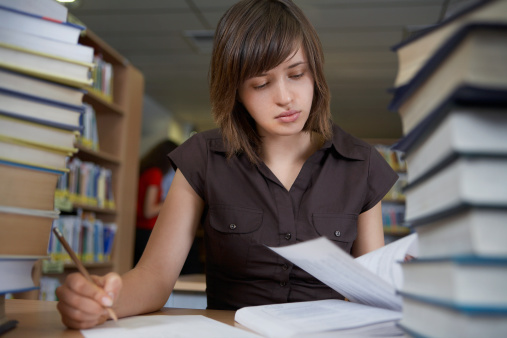
\includegraphics[width=0.25\textwidth]{Grafik/FoodPlanner/PersonaAnneMadsen}
	\label{PersonaHenrikJensen}
\end{figure}
\begin{itemize}
	\item Age: 18
	\item Relational status: Single
	\item Children: None
	\item Occupation: Student
	\item Preferences: Likes to spend time in the kitchen to prepare a good fresh meal with vegetables
\end{itemize}
-Anne has classes till late afternoon, after school Anne has a specific shopping list based on what she has to buy to make food for dinner.

-Anne does not know where to find the cheapest groceries which she finds slightly annoying, so she keeps shopping the same place as she has always done.

-When Anne is done shopping she decides that it is too dangerous to ride her bike with a bag of groceries hanging of her handlebar. So she decides to pull her bike home.

-When Anne finally gets home the trip from school to home has taken so long that it is time to make dinner.

-After dinner she cleans the plates, and gets ready to prepare her homework for the next day. 

\chapter{Problem Domain}
In this chapter the reality the user is going to see will be described. This reality is constructed of the areas which the system is going to administrate, monitor or control. Descriptions of classes, objects, structures and behaviours will be made throughout the chapter.


\section{Classes}\label{ClassesLabel}
In this section a list of classes will be presented. The classes described are those which have been chosen through a class candidate analysis.

\subsection{Physical}
\begin{itemize}
\item \textbf{Product:} This class is used to identify different ingredients for the recipes with information such as food type and expiration date. This class is essential for the program and will be used frequently.
\item \textbf{Recipe:} This class holds information about the ingredients and instructions on how to cook the meal.
\item \textbf{Scheduled Meal:} This class contains information about a recipe and when it is scheduled to be cooked.
\end{itemize}

\subsection{Persons}
\begin{itemize}
\item \textbf{User:} This class contains information about the preferences of a specific user, and will allow the solution to synchronise/share data with other users or devices.
\end{itemize}

\subsection{Places}
\begin{itemize}
\item \textbf{Shop:} This class holds information about the location of specific groceries and discounts.
\end{itemize}

\section{Events}
In this section a list of events will be presented. The events described are those which have been chosen through an event candidate analysis. The events and what trigger them are listed below.
\subsection{Consumption}
\begin{itemize}
\item \textbf{Product bought:} A shopping list have been completed. The items bought will be added to an inventory.
\item \textbf{Product removed:} A meal have been prepared and the product should be removed from the inventory, or have an subtraction from its original volume/quantity.
\item \textbf{Product expired:} When a product reaches its expiration date, it should be removed from the inventory and thrown out.
\end{itemize}

\subsection{Planning}
\begin{itemize}
    \item \textbf{Recipe scheduled:} When a recipe is scheduled for a date in the meal plan.
    \item \textbf{Recipe removed:} When the user removes a recipe which was scheduled for a date in the meal plan.
    \item \textbf{Shopping list item added:} When a recipe have been scheduled in the meal plan, missing ingredients from the inventory are added to the shopping list.
\end{itemize}

\subsection{Preferences/settings}
\begin{itemize}
\item \textbf{Preference changed:} When the user navigates to a settings menu to exclude products from the system, due to allergies, diets or preference.
\end{itemize}

\section{Event Table}
\Cref{tab:EventTable} shows an event table that have been constructed in order to get an overview of the relations between classes and events. The event table allows for a better judgement of which classes are relevant in the program. A plus (+) in the table indicates, that an event can occur zero or one time, whereas a star (*) indicates that an event can occur zero or more times.

\begin{table}[H]\centering
    \begin{tabular}{|r|c|c|c|c|}
        \hline
        ~                                      & Product & Recipe & User & Meal\\ \hline
        \textbf{Consumption}                   & ~       & ~      & ~    & ~   \\ 
		    Product added                          & +       & ~      & ~    & ~   \\ 
        Product removed                        & +       & ~      & ~    & ~   \\ 
        Product expired                        & *       & ~      & ~    & ~   \\ 
        Product unexpired                      & *       & ~      & ~    & ~   \\ 
        Product quantity changed               & *       & ~      & ~    & ~   \\ 
        Product expiration changed             & *       & ~      & ~    & ~   \\ 
        \textbf{Planning}                      & ~       & ~      & ~    & ~   \\ 
        Shopping list item added               & +       & ~      & ~    & ~   \\ 
        Meal added                             & ~       & +      & ~    & +   \\ 
        Meal removed                           & ~       & +      & ~    & +   \\ 
        Meal rescheduled                       & ~       & +      & ~    & +   \\ 
        Meal participants changed              & ~       & ~      & ~    & *   \\ 
        Meal Date changed                      & ~       & ~      & ~    & *   \\ 
        \textbf{Other}                         & ~       & ~      & ~    & ~   \\ 
        Preference changed                     & ~       & ~      & *    & ~   \\ 
		    Recipe found                           & ~       & *      & ~    & ~   \\ 
		\hline    
    \end{tabular}
    \caption{An event table for the program} 
    \label{tab:EventTable}
\end{table}
\section{Event Traces} \label{EventTraces}
This section will present a statemachine diagram for each class. Each statemachine diagram is the result of examining each class, with a focus on identifying the different states of the class' objects and the events, which effects the objects and changes their state. An event can happen without changing the state of the class e.g. on \cref{MealClass} the \textit{Change scale} event will not lead to a new state for the meal class object.  

Each class examination first shows a few of the event traces that were formulated for the specific class. The relationship between the classes and events are described in \cref{tab:EventTable}. The event traces will be used to model the statemachine diagram for the specific class. The event traces and statemachine diagrams are created to get a better understanding of the dynamic in the problem domain. It is possible to use the event definitions in \cref{EventsSection} for a better understanding of each event, if the event behaviour is not clear from the event name.   

\subsection{Food Class}
Some of the event traces used to understand the behaviour of this class are:
\begin{itemize}
	\item \textit{Added} -> \textit{Expired} -> \textit{Quantity changed} -> \textit{Removed}.
	\item \textit{Added} -> \textit{Quantity changed} -> \textit{Expired} -> \textit{Quantity changed} -> \textit{Unexpired} -> \textit{Removed}.
	\item \textit{Shopping list item added} -> \textit{Added} -> \textit{Expired} -> \textit{Removed}.
	\item \textit{Shopping list item added} -> \textit{Shopping list item removed}.
\end{itemize}

This class also has some event traces which are not legal e.g. 
\textit{Shopping list item added} -> \textit{Expired}.

\begin{figure}[tbhp]
	\centering
	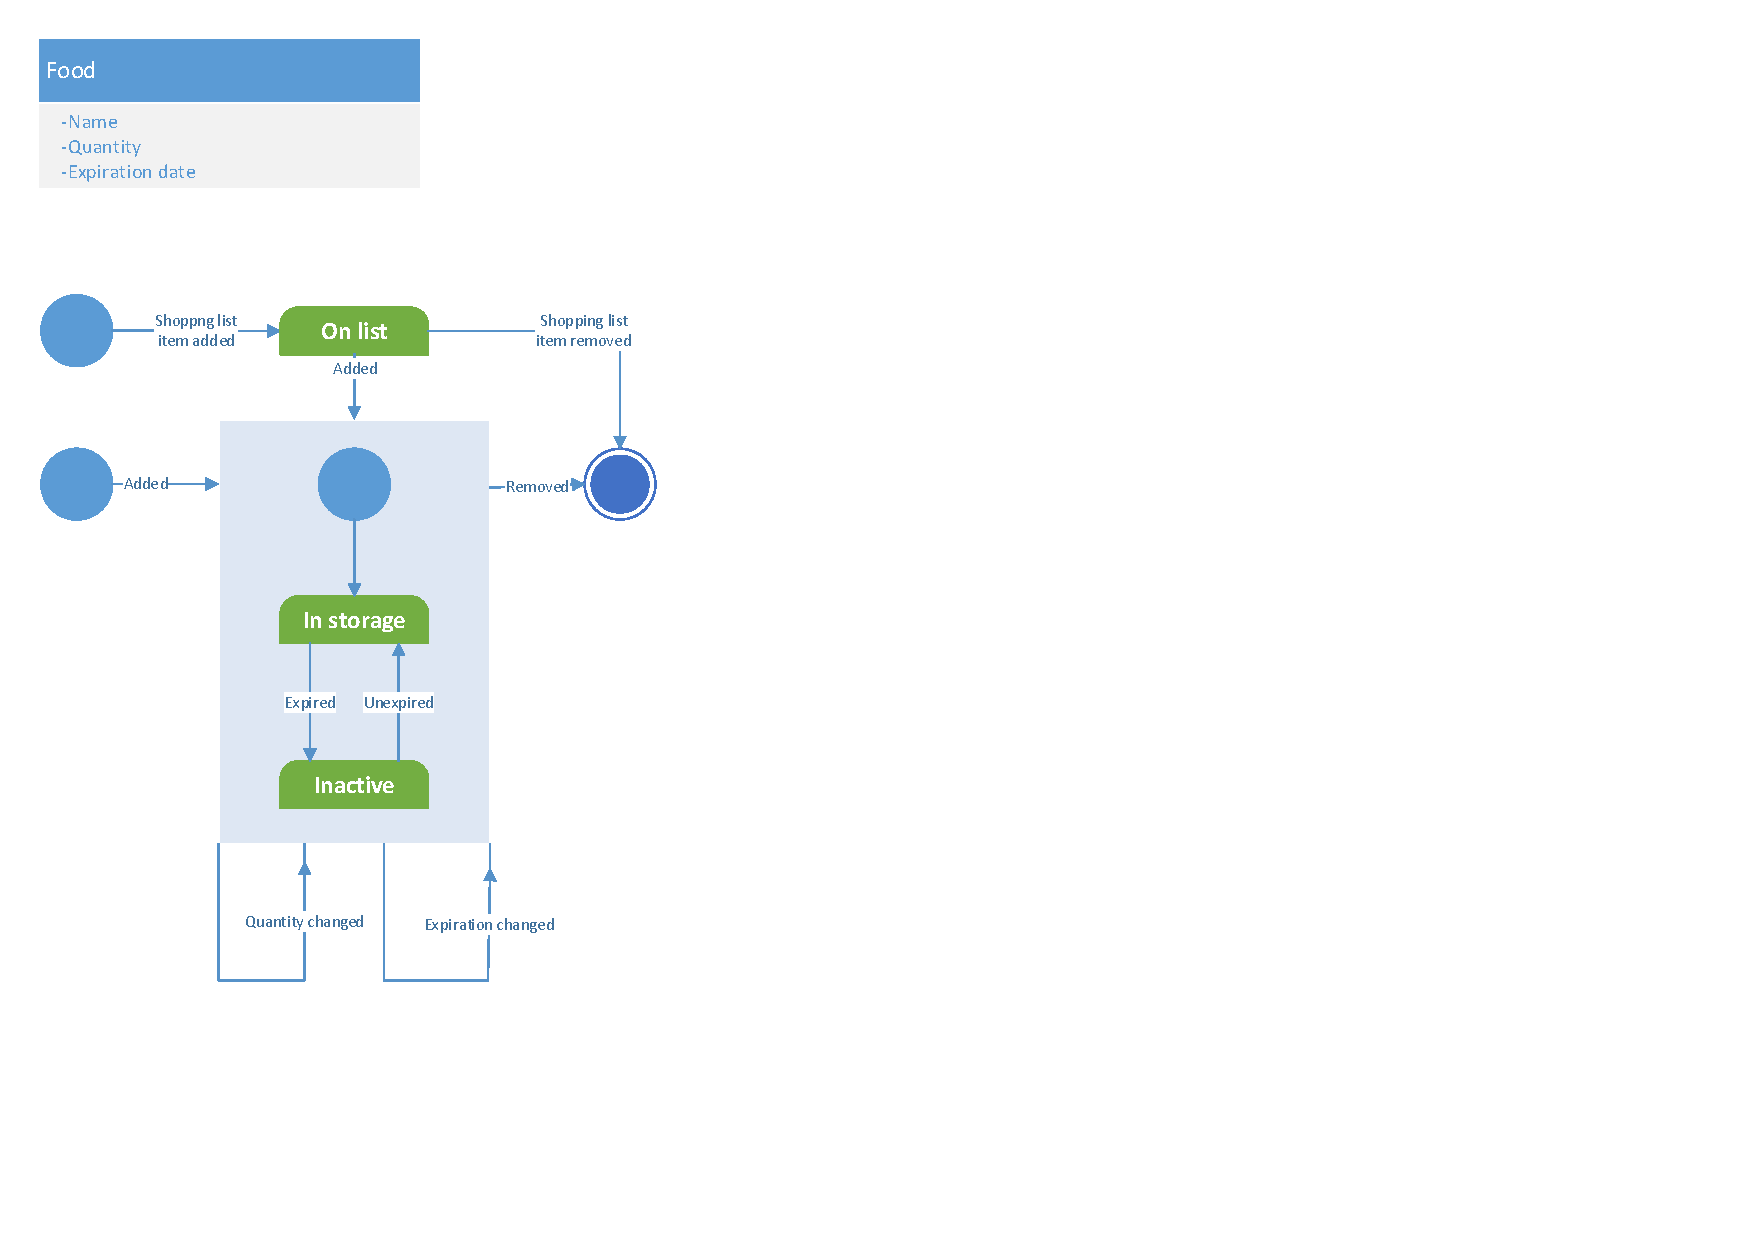
\includegraphics[clip=true, trim=0.5cm 4cm 18.5cm 0.5cm,  ]{Grafik/FoodPlanner/Food.pdf}
	\caption{Statemachine diagram for the Food class.} \label{FoodClass}
\end{figure}
An object of this class can be instantiated when the user either adds a shopping list item or adds a food item directly to their inventory. The two starting events for this class are therefore \textit{Shopping list item added} and \textit{Added}. The two start events sets the object's state to either \textit{On list} or \textit{In storage}. The On list state can be changed by the Add event, which sets the state to In storage, or by the \textit{Shopping list item removed} event, which terminates the object. The object can also have the state \textit{Inactive}, which can be set by the \textit{Expired} event and reset to the In storage state by the \textit{Unexpired} event. It is possible for an object in both the In storage and Inactive state to be effected by the \textit{Quantity changed} and \textit{Expiration changed} event, without changing the object's state. These two events can be iterated throughout an object's lifetime. The object can also be terminated from the In storage and Inactive state, by the \textit{Removed} event.   

\subsection{Meal Class}
Some of the event traces used to understand this class are:
\begin{itemize}
	\item \textit{Meal added} -> \textit{Change scale} -> \textit{Meal prepared}.
	\item \textit{Meal added} -> \textit{Change date} -> \textit{Meal prepared}.
	\item \textit{Meal added} -> \textit{Day passed} ->\textit{ Reschedule meal} -> \textit{Meal prepared}.
	\item \textit{Meal added} -> \textit{Change scale} -> \textit{Change date} -> \textit{Change scale} -> \textit{Meal prepared}.
\end{itemize}

An example of event traces that are not legal for this class are: \textit{Meal added} -> \textit{Day passed} -> \textit{Change Scale}.

\begin{figure}[H]
	\centering
	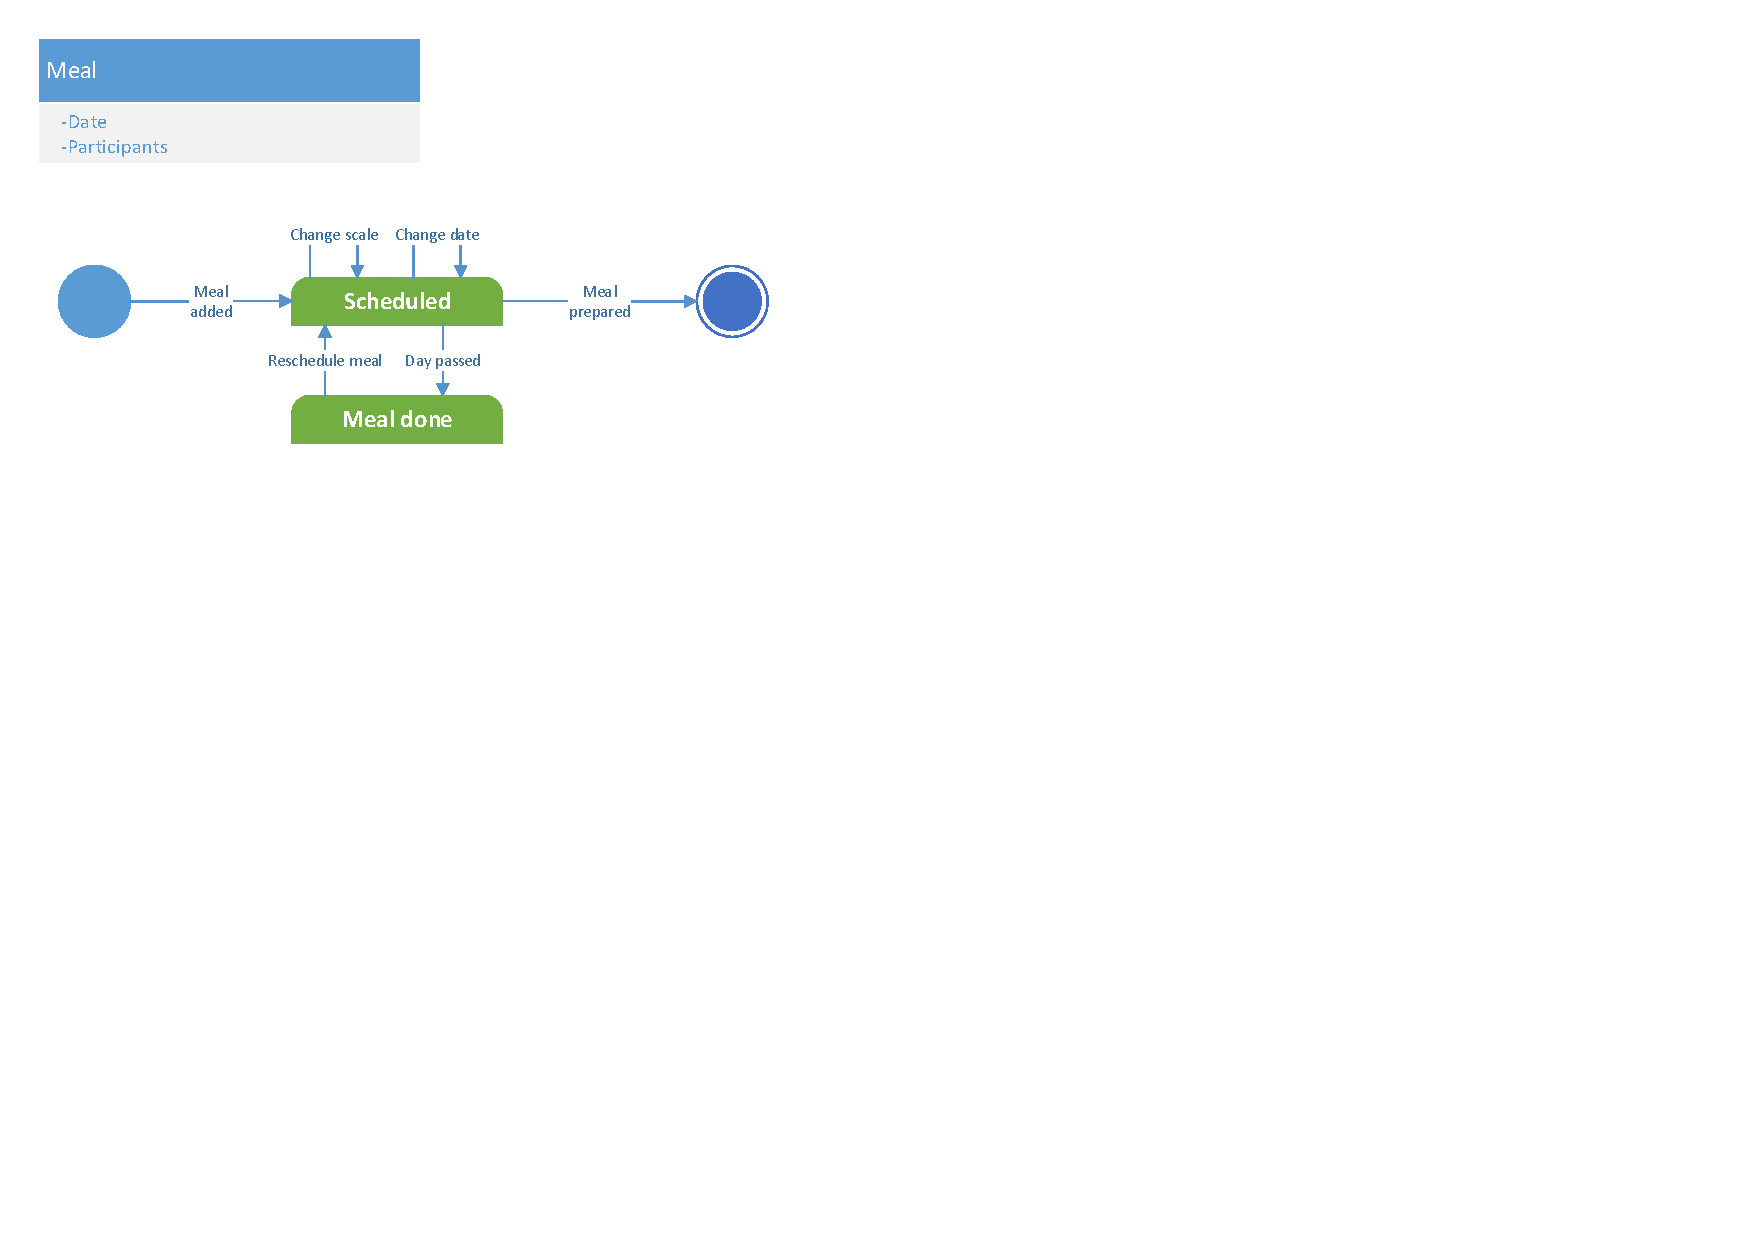
\includegraphics[clip=true, trim=0.5cm 13cm 16.5cm 0.5cm]{Grafik/FoodPlanner/Meal.pdf}
	\caption{Statemachine diagram for the Meal class.} \label{MealClass}
\end{figure}

An object of the meal class can be instantiated by the \textit{Meal added} event, and this sets the state of the object to \textit{Scheduled}. The events \textit{Change scale} and \textit{Change date} can be iterated throughout the object's lifetime, and does not change the state of the object. The object can also have the \textit{Meal done} state, which can be set by the \textit{Day passed} event and reset to the Scheduled state by the \textit{Reschedule meal} event. The object can only be terminated by the \textit{Meal prepared} event.

\subsection{User Class}
Some of the event traces used to better understand the events and flow of the User class are:

\begin{itemize}
	\item \textit{User registered} -> \textit{Preference added} -> \textit{Preference added} -> \textit{User deleted}.
	\item \textit{User registered} -> \textit{Preference added} -> \textit{Preference removed} -> \textit{User deleted}.
\end{itemize}

An event trace which is not legal for this class could be \textit{User registered} -> \textit{Preference removed} -> \textit{User deleted}.

\begin{figure}[H]
	\centering
	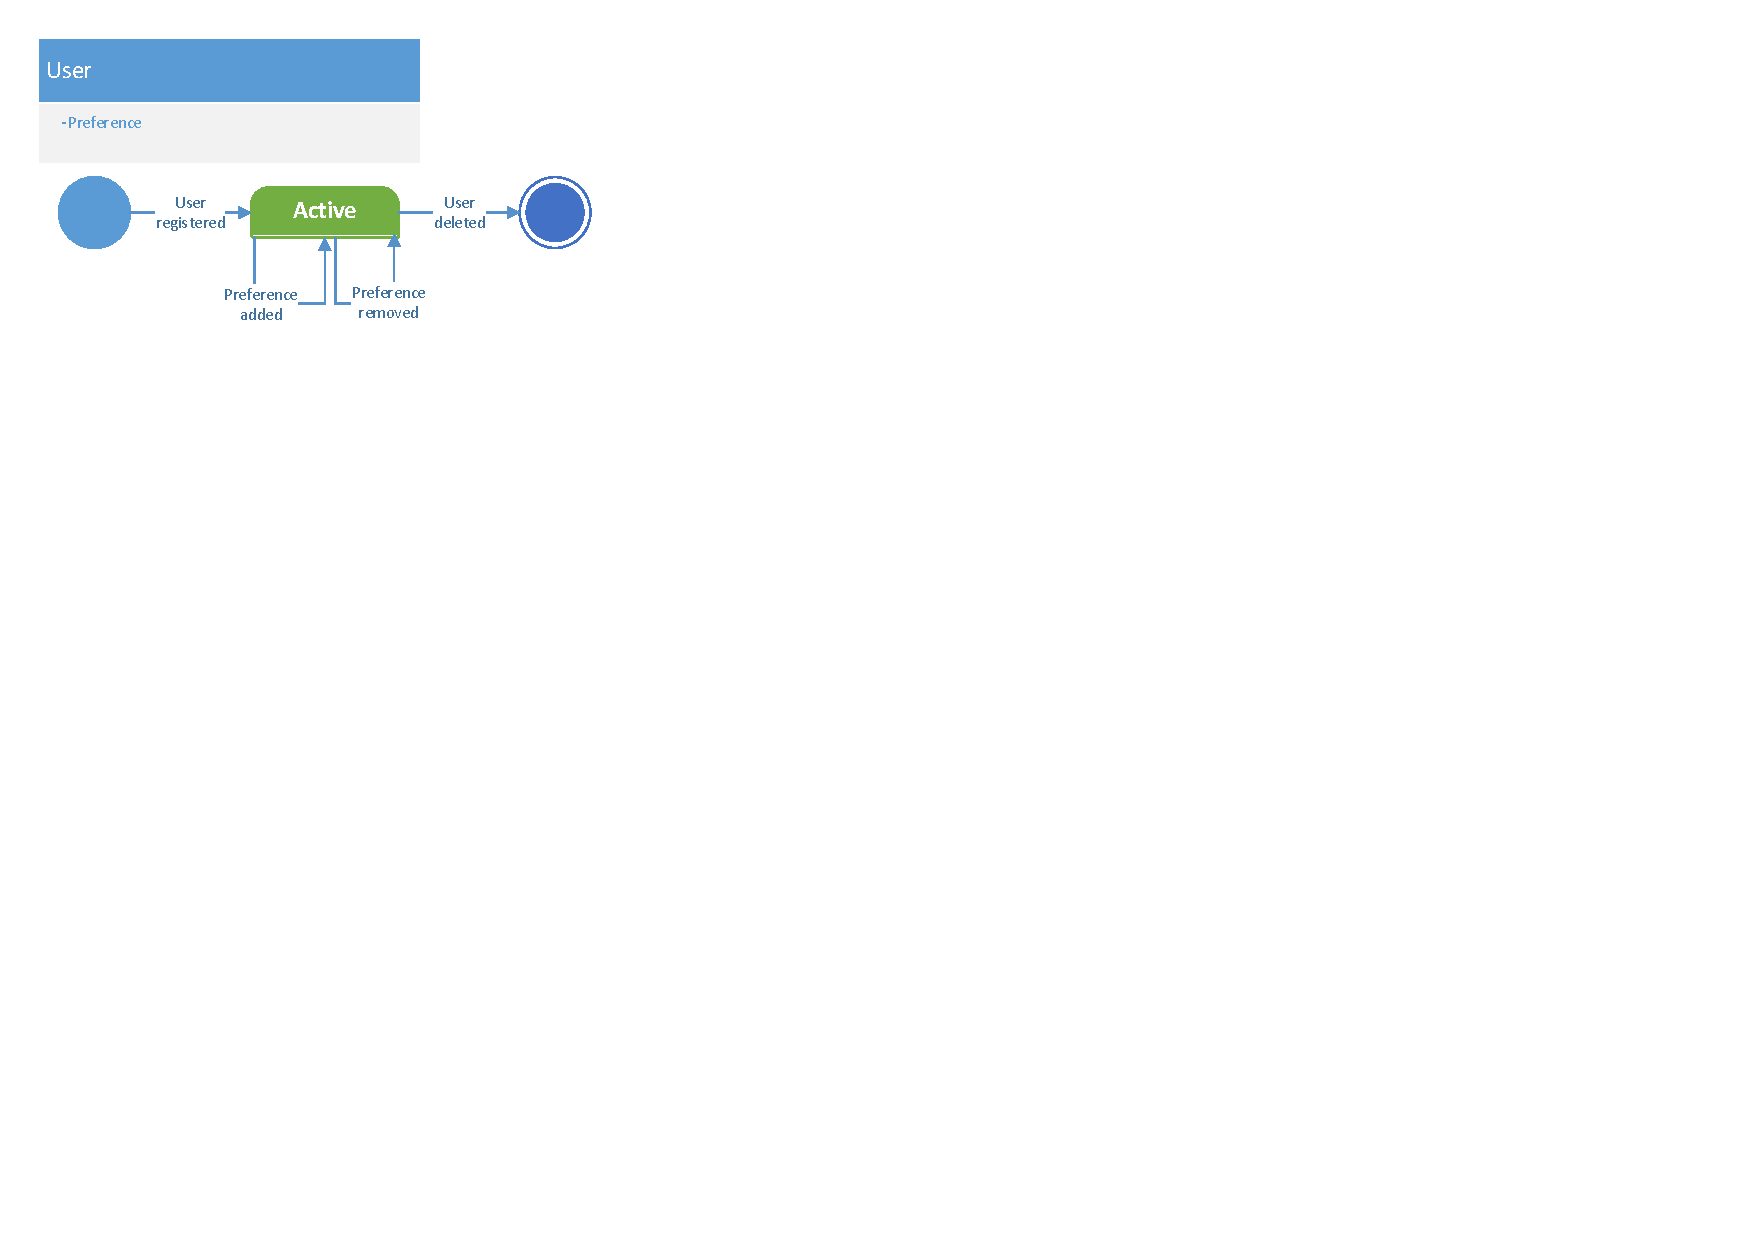
\includegraphics[clip=true, trim=0 14cm 5cm 0]{Grafik/FoodPlanner/UserSettings.pdf}
	\caption{Statemachine diagram for the User class.} \label{UserSettingsClass}
\end{figure}

This class can have an object instantiated by the \textit{User registration} event, and this event sets the object's state to \textit{Active}. From this state the \textit{Preference added} and \textit{Preference removed} event can be iterated throughout the object's lifetime. The object can only be terminated by the \textit{User deleted} event.


\subsection{Recipe Class}
Some of the event traces used to understand the Recipe class are:
\begin{itemize}
	\item \textit{Recipe added} -> \textit{Recipe removed}.
	\item \textit{Recipe added} -> \textit{Recipe found} -> \textit{Meal added} -> \textit{Meal removed}.
	\item \textit{Recipe added} -> \textit{Recipe found} -> \textit{Recipe found} -> \textit{Meal added} -> \textit{Meal removed}.
\end{itemize}

One of the event traces which are not legal for this class are:\textit{ Recipe added }-> \textit{Recipe found} - \textit{Meal removed}.

\begin{figure}[H]
	\centering
	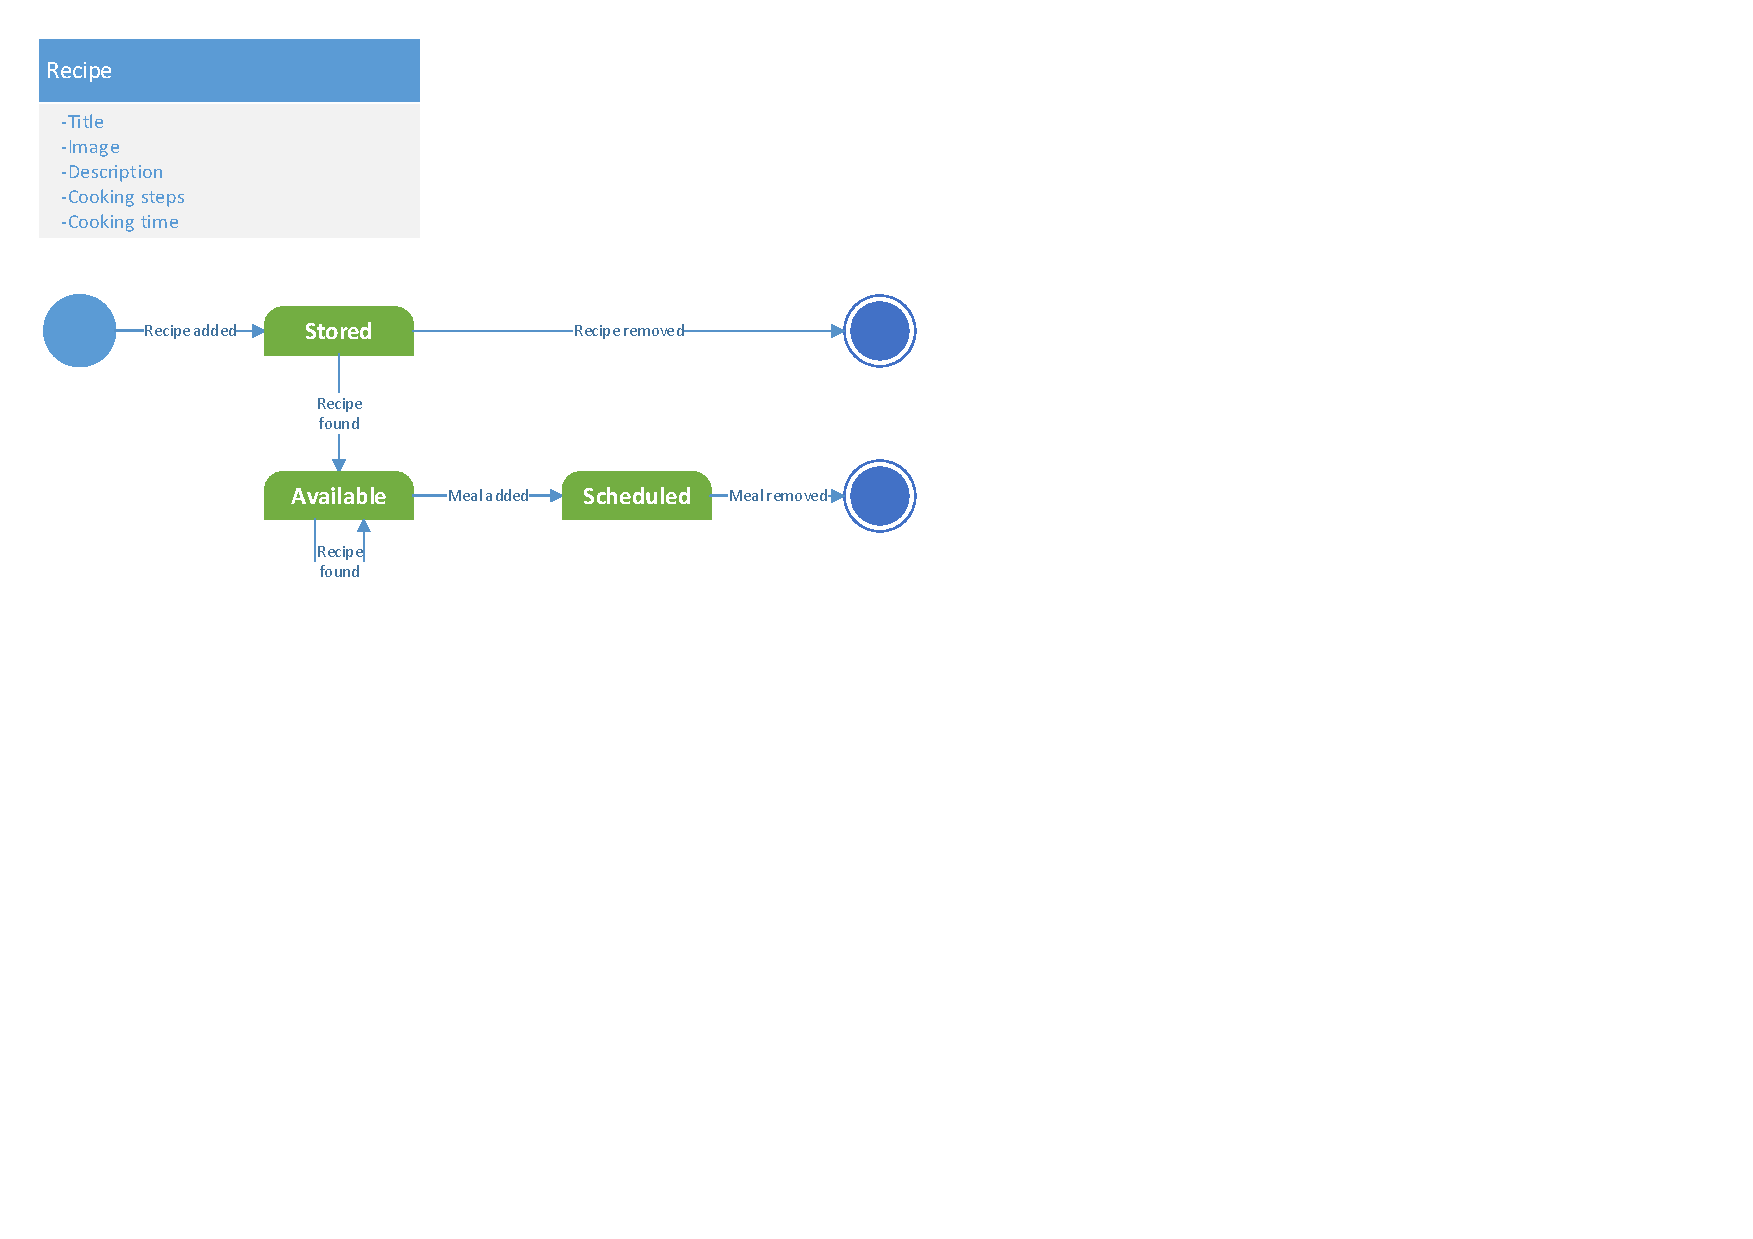
\includegraphics[clip=true, trim=0.5cm 11cm 14cm 0.5cm]{Grafik/FoodPlanner/Recipe.pdf}
	\caption{Statemachine diagram for the Recipe class.} \label{RecipeClass}
\end{figure}

An object of the Recipe class can only be instantiated by the \textit{Recipe added} event, and this event sets the state of the object to \textit{Stored}. From this state the \textit{Recipe removed} event can terminate the object. The \textit{Recipe found} event can change the object's state from Stored to \textit{Available}. The same event can also be iterated in this state, without changing the state. The \textit{Meal added} event can change the object's state to \textit{Scheduled}. From this state the \textit{Meal removed} event can terminate the object.

	\part{Design}
		\chapter{PACT}
\section{PACT analysis} \label{PACTAnalysis}
In this section, a PACT (People, Activities, Context \& Technology) analysis will be conducted in order to acquire an understanding of how people will use and interact with the system.\fxnote{Describe PACT in this into, how it is used and why it is}
\section{People}
Everyone needs food, and many also have to buy and make it themselves. There are many ways to prepare a meal, and people have different preferences of what they eat and why. In this analysis the focus will be on the social, physical and psychological differences between people and on a description of their different motives and preferences. This description will be used to get an idea of who could benefit from a system, that would help them organize grocery shopping and preparing meals more efficiently.

\subsection{Physical differences}

People have different physical abilities. Some people have bad vision, some have bad hearing, and so on with a lot of different physical conditions, and taking this into consideration is an important aspect of a PACT analysis.

Looking at the ergonomically aspects of the application is not necessary, since the ergonomics are decided by the company who creates the device that the application run on. Therefore ergonomics are not something that can be affected by the application.

\subsection{Psychological differences}

People vary in the way that they function psychologically. But some of the common traits to look at when designing software are:

\begin{itemize}
    \item The meaning of buttons
    \item Not too hard to remember instructions
\end{itemize}

The meaning of buttons is very important because depending on where the software will be released, buttons mean different things. Since the food planner application is designed to be released in Denmark, it is therefore important that the Danish people will perceive the buttons correctly.

It is also important that no instructions or commands are too long, because it will be hard to remember for some people, and when making a product you must take the weakest user into consideration when looking who to design the product for.

\subsection{Social differences}

People have different requirements for a product, and it is therefore important for the developer to make sure that everyone can get what they desire from the product. Therefore some groups of people with social differences will now be mentioned.

\subsubsection{People following a special diet, or having specific wishes for food plans}
People that are on a specific diet needs to buy food based on the diet, and sometimes prepare it in a specific way.
Some examples of these people could be:
\begin{itemize}
\item Athletes (Bodybuilders)
\item Vegans/vegetarians
\item Organically minded
\end{itemize}

\subsubsection{People who want to save time when planning cooking, doing the groceries and preparing the food} 
If people do not plan what they are going to eat throughout the week, they often have to buy groceries every day, and maybe the food they are preparing takes a longer time to cook than they expected. In this case, an organized foodplan based on how long time it takes to prepare a meal and what groceries you have, could help save time in the everyday life. Examples of people who can benefit from saving time because of tight schedules can be:
\begin{itemize}
\item Students
\item Parents
\item Families
\end{itemize}

\subsubsection{People who want to be social while eating}
When people wants to get together and eat for different occasions, it could be beneficial if they plan the meal based on the preferences of the people involved. The reason why people would like to be social while eating could be just wanting to talk to others, but also to save money by preparing bigger meals, and people trying to have less food waste by cooking together. Examples of people who would like to be social while eating can be:
\begin{itemize}
\item Social eaters, people who only get together to eat a meal together
\item Students
\item Parents
\item People with a tight or small budget
\item Students
\item Parents
\end{itemize}

Some people might only want to eat with people of the same interests and food habits, for the same reasons as the people wanting to be social, but finds it easier if cooking together with people of the same interests and habits. These people include:

\begin{itemize}
\item Vegans/vegetarians
\item Organically minded
\item Social eaters
\end{itemize}

\subsubsection{Comparison}
It is common for all the described people that they could save time and/or money by planning their grocery-shopping and meals. A system would have to be fast and easy to use, so that the time spent planning does not exceed the time it would take to plan a meal completely manual. The system could automate tasks for the user, for example by recommending recipes and keeping track of what food they already have at home. It must be easy for the user to input the groceries, and not become a burden, preferably this should be fully automated, for example by adding groceries from a shopping list that a user used when shopping, or semi-automated by allowing the use to scan the product barcode.
\section{Activities}
To see in which context the program will be used, we first look at the activities associated with using the program. The activities have been split into two categories, what happens \textit{inside} and \textit{outside} of the home.

In the home:
\begin{itemize}
\item The program will be used to manage the food supply, by;
	\begin{itemize}
		\item Viewing a list of the stored groceries
		\item Updating the list, by adding or removing groceries that could have been used, or groceries that have gone bad
		\item "Flushing" the stored groceries. This should be done when the program is initiated for the first time or after a long period of inactivity
		\item Create a shopping list of the groceries needed for the planned meals
		\item Search for recipes
		\item Add new or modified recipes
	\end{itemize}
	Furthermore it should be in the home that preferences are set, which could be groceries you want to ignore, because;
	\begin{itemize}
		\item You do not like them
		\item You are allergic
		\item The grocery is not associated with a certain diet
	\end{itemize}
	Certain recipes will require the use of certain kitchen tools, therefore you would want to;
	\begin{itemize}
		\item View what tools are needed
		\item Be able to check if you have the kitchen tools
		\item Associate kitchen tools with a specific recipe
	\end{itemize}
	\item While cooking the meal, you would want to follow a recipe while cooking, which mean you might have to interact with the program during the cooking
\end{itemize}

Outside the home:
\begin{itemize}
\item While shopping for groceries, it is necessary to keep track of the shopping list, to see what should be bought.
\item If a new recipe is wanted on the fly, the shopping list must be updated
\end{itemize}

Frequent activities such as looking for a recipe should be easy to do, but some activities such as flushing the stored groceries should be easy to learn. This could be done by having a walkthrough when a user tries to do this particular activity. The program should also have easy navigation options to allow for mistakes to happen, such as going into undesired program pages, and still be able to get back on track. If the user is interrupted and have to pause their usage of the program, the user should be able to continue later from the same point. This is relevant if they are making a grocery list or a new recipe. These documents should have a save and edit function in order for the user to pick up on their work later.

The response time could become a point of frustration for the user if they want to lookup an online recipe and the response time is more than five seconds. As the recipes are available online there is a risk of high latency between a user's device and the server containing the recipes. A workaround for this could be to have a local version of the recipe database, and only have the device to synchronise the two databases once in a while.

The user is able to add or edit recipes and groceries to lists, and will therefore need an method of inputting alphabetic data into the program. Since the solution is minded to be on a handhold or mobile platform, a keyboard is not optimal as it will be frustrating to carry around. A small integrated keyboard, like the one a BlackBerry has\cite{blakBerry}, would not work either as it will get dirty when used in the kitchen. For example if the user is baking and want to type on the keyboard, flour could get in between the buttons, which would be difficult to clean. A touch display can simulate a keyboard and easily be cleaned with a towel and, and is therefore the best option for this solution. Voice recognition could also be a possibility, but outside noise will be too big of a nuisance. A lot of noise could interfere with the program when the user is in a mall or using kitchen tools such as a blender, or if they are boiling water.
\subsection{Context}
In this section we look at the context in which certain activities are performed. The examined contexts are the physical environment, and the social context.

\subsubsection{Physical environment}
Using the program in different locations will have different impact on the user experience. Having the program on a device will set some limitations, as the user will have to interact with the program, during different situations.
\begin{itemize}
\item With the households inventory stored in the program, a user will not have to be home, to see what is missing, if he/she chooses to add another recipe.
\item While shopping, one hand must be free, to check which items that has been put in the basket, and what else must be bought.
\item While cooking at home, an ingredients list could be revisited, or a cooking guide will have to be followed, with greasy hands this kind of interaction will be difficult.
\end{itemize}

\subsubsection{Social context}
The program can be used in different social context.
\begin{itemize}
\item If more than one person share the same food plan, they must both have access to the program, and if it is handled on their personal devices, synchronization is necessary.
\item The program can be used by only one person and on one device only, therefore synchronization might be a nuisance instead of a trait for this type of user.
\item With an online database of recipes, it would be possible to add new recipes and share these, with other users.
\end{itemize}\fxnote{Conclude on this plz!}
\subsection{Technologies}
In the technology part of the PACT analysis, there is looked upon input, output and communication, which will be examined by the pros and cons of different relevant technologies, with a focus on tablet and smartphone related technologies.

\subsubsection{Input}
The program should function as a planning tool, and include a shopping list, therefor the final platform will likely be tablets or smartphones, since they are more mobile than a laptop, and therefore there might not be any external plug-in devices that are going to be used for the solution. This means that the available input technologies are:
\begin{itemize}
    \item Cameras
    \item Microphones
    \item Touchscreens (includes multi-touch)
    \item Physical buttons
\end{itemize}

\paragraph{The camera} can be used to input pictures, video or barcodes. Pictures and videos can be useful when the user adds content to the program, such as creating a recipe or adding a instructional videos. It is possible to get applications on some popular mobile operating systems such as iOS, Android and Windows Phone \cite{barcode_Phones}, that scan traditional barcodes and QR codes. Being able to read these codes could become useful if there are any relevant data on the 2D barcodes that needs to be transferred to the device. This data could be the item type or expiration date \cite{barcodeInc_FAQ}.           
    
\paragraph{The microphone} can be used to input audio into the device. This can be useful if the users hands are occupied and they need to do some simple interaction with the program. These interactions would be made possible by the use of voice recognition software.

The touchscreen is easy to use and can be found in tablets and smartphones. The user can press the screen with their finger to interact with the program. Some touchscreens also enables the use of multi-touch technology, this enables more than one finger to be used when interacting with the touchscreen, this is often used for operations such as zooming (pinching) and rotating of pictures and text. This is useful in the general use of the program.

Physical buttons on the device could be used to navigate throughout the program, together with the standard functionality e.g. volume control. The amount of programmable buttons varies from device to device, the iPhone/iPad does not allow secondary functionality on their buttons. Some devices that run the Android OS allows for second functionality\cite{android_Rebind}, and should therefore be considered when designing the program.

\subsubsection{Output}
The list of output technologies are:

\begin{itemize}
    \item Screen
    \item Speakers
    \item Vibration
\end{itemize}

The screen is used for visual display and visual feedback. Screen technology is useful to display large amount of information to the user.
The size of the screen must be taken into consideration when displaying information such as screen elements (e.g. buttons) and/or text.
Devices such as a laptop screen or desktop monitor can display many elements and large quantities of text.
Large amounts of text can require pinching and scrolling making it hard to read. Large clutters or quantities of elements can also be hard to navigate through.
It can be useful for all screen sizes to use symbols to show what elements can do instead of using screen space on unnecessary elements.

Speakers and/or vibration can be used in conjunction with the screen to give different kinds of feedback simultaneously.
Speakers and vibration are especially useful to give the user feedback in situations where the screen of the device is not viewable.
The speakers are helpful in situations were there are no physical contact with the device but it is still in hearing range.
This could be applied in many home situations were the user might not have the device with them, or they can not see the device.
Vibration is useful when the user has physical contact with the device or in situations where sound might be hard to hear, or is disabled.
This could be useful in crowded environments such as a shopping mall.     

\subsubsection{Communication}
Communication means how the solution are supposed to communicate with the internet and other users. The list of technologies is:

\begin{itemize}
	\item Wi-Fi
	\item Telephone networks
    \item Database
\end{itemize}

A Wi-Fi connection is a wireless connection to the internet.
This is a useful technology because all modern tablets and smartphones has Wi-Fi technology.
Wi-Fi can be used to access data that are stored on other devices which are not used by a user such as a server.
It can also be used between devices on the same network to synchronize changes in the program.    
%
%The Wi-Fi of the tablet or cell phone are used for connecting to the internet, to be able to synchronize the changes in the program so it can be viewed on a different device. But the Wi-Fi is also used for accessing databases so information about products can be accessed.

Telephone networks is used for the same reason as Wi-Fi. Though some mobile devices does not allow for the use of telephone networks.
Some tablets are cheaper when they only provide Wi-Fi technology, therefore both Wi-Fi and mobile networks are technologies worth considering.

A database can be used to store data on and the data can be accessed via the internet.
This is useful because a database can store larger amounts of data than a mobile device.
 
\subsubsection{Conclusion}
Many different technologies are required to be considered when doing a PACT analysis, the technologies needed for the food planner application is from the three categories; input, output, and communication.
The technologies ranges from physical buttons, to the Wi-Fi element needed for the synchronization of the data. The chosen input technology that is going to be used is the touchscreen, as it is already widely used and works well with the solution. The chosen output technology is going to be screen display together with sound. The screen will hold the necessary text and visual information, where the sound may be used for alert or notifications. The communication technologies will going to be all of the previously described. Wi-Fi is useful for communicating with the server and other devices and the telephone networks can be used to transfer data when the user is outside of their home or work. The database will be used for holding a large amount of somewhat trivial data, such as the recipes. By having the recipes on the database the user saves room on their data storage device.


%\subsection{Young couple}

\begin{itemize}
\item Elena Miller \& Jacob Collins
\item Have been together for a few years
\item Elena is still under education. and Jacob is new in job
\item They live together in a small rented house
\end{itemize}
\begin{minipage}{2}
\begin{itemize}
\item 1
\end{itemize}
\begin{itemize}
\item 2
\end{itemize}
\end{minipage}
\chapter{Scenario-based design}
\section{Domains}
Domains are important to look at to be able to make the best possible design for the interface of the system. Domain is defined as the different aspects of the program, and both large and small domains will be described.

\subsection{Planning}
Planning is the largest domain of the project, as the software developed is focused on planning meals and a creating a shopping list. Furthermore is planning the primary aspect of the project, as the analysis has concluded that food waste can be reduced by planning meals ahead.

\subsection{Grocery shopping}
Grocery shopping is one of the small domains, as the shopping itself is not something that the software takes into consideration. BY having the software generate a shopping list, for the user to follow, impulse shopping will be reduced, as concluded in the analysis.

\subsection{Cooking}
Cooking is also a small domain. The software gives the user a recipe, where in the quantity of needed ingredients can be changed depending on how many persons the meal will be prepared for.

\subsection{Food inventory administration}
The last domain of the project is food inventory administration. The software is keeping track of the users inventory, so the user can have an easy overview of what is present in the home, but also to be able to calculate that needs to be bought to be able to cook the recipes that are on the meal plan.
\subsection{Design Requirements} \label{DesignRequirements}
When analysing the interviews in \cref{InterviewAnalysis}, conceptual scenarios in \cref{conceptualScenarios}, the PACT analysis in \cref{PACTAnalysis} and the personas \cref{PersonasAppendix}, some design requirements are discovered. These requirements have been listed in the appendix, \cref{RequirementsAppendix} and are later included in the definition of a scenario corpus. Furthermore the long list of requirements have been sorted into the same domains as can be found in scenario corpus, \cref{ScenarioCorpus}, but also includes a list of more general requirements followed by a list to requirement actions, as well as a limited list of technologies, which can be used. Some Requirements can be placed in more than one domain, but is only be listed in the domain that seems most ideal.
\subsection{Stories} \label{UserStories}
All products and processes of the design method springs from the product \textit{Stories}, which are shown below. The stories are written by different persons who have described their last shopping situation.
The stories vary in detail but can all be used to find different actions, requirements and problems, which is some of the aspects that are used in the following processes and products of the method.

\subsubsection{Person A}
\begin{quote}
I have invited guests for dinner Monday evening. We were having kale and ham, both something I had in the freezer, actually I had two hams in the freezer, because I bought one on a sale the day before, and that way I would be sure that there was enough meat, in this new and bigger ham. The only thing missing for the evening meal is now two litres of skimmed milk, so off I went to the grocery store, with my dog  on a leash. We walked to the closest store, which also happens to be a big store. When I entered the store, I began to doubt if the ham really was big enough, so I looked in the fridge with sausages.
I found a Christmas sausage on sale, and thought "Better safe than sorry" when I put the sausage in my basket, furthermore I thought to myself that any spare meat could be used as cold cuts, in the days to come. I headed for the two litres of milk, and then the checkout. On the way I passed the vegetable area, and saw dried figs, "Who can resist such a thing, so into the basket with those as well". I got through the checkout, and past the bakery on my way out to the dog, "The dog!", I could not forget to get her something, so I went back to the bakery to get a sausage roll. They had a sale, where you could buy 5 rolls, "So why not do so?".
\end{quote}

\subsubsection{Person B}
\begin{quote}
Last time I went shopping was when we in the household were to eat together. Another person in the household looked through the kitchen, to find out what was missing, and then told me; butter, potatoes, carbonated soft drinks, and dessert. I went to the closest store, and bought what was needed. When I returned to the apartment I decided that we should have the drink "White Russian" as desert, we had all we needed except milk, so off I went again, thinking that this extra trip could have been avoided if we had talked about which dessert I was actually meant to get, before I went for the first trip.
\end{quote}
 
\subsubsection{Person C}
\begin{quote}
Knowing that I want to shop the day after this day, I place a piece of paper on the table, and during the day, every time I remember basic stuff that we need, I write it down, things like, paper towels, rice, soap, and so forth. Later during the day I sit down to look through recipes to figure out what to have for dinner the next couple of days. I match recipes with what we already have at home, so that we can clear some of the storage, and in that way save some money, now that we are close to Christmas, and the budget therefore is a bit more tight, than normal. Because I based the meals on what we had at home, the shopping list did not get that long, therefore I was determined only to have to go to one store, the day after. Next day the planned shopping did not go as anticipated since both my husband and I had to work until late that day, therefore, I only went to get the most critical items on the shopping list, making an easy dinner for the evening, and food for the kids to bring as lunch the following day. During the shopping I remembered that my youngest child had to bring an advent present to school the next day, so I bought this as well and the rest of the shopping list had to wait until tomorrow.
\end{quote}

\subsubsection{Person D}
\begin{quote}
The last time I had to go shopping, was to get groceries for a Christmas party. My boyfriend and I had to get cabbage and cream to make kale, and we had to get marinated herring. Preferably we wanted to get herring marinated in tomatoes, and the cream had to be organic, because I am allergic to milk products that are not organic. Because of these requirements we chose to shop in one of the biggest malls, in the city. But to our big surprise, they did not have any marinated herring other than the ordinary, and they only had $1/4$ litre organic cream. Because of this this we therefore chose to get it in another store. Before we got to the checkout I found a Christmas gnome costume, for my niece, which I wanted to get for her, and to go with this costume we had to get a pair of matching tights as well. Furthermore my boyfriend found a cheap bathrobe, which he has wished for, for a long time and he therefore chose to buy it. We now went to the next store, to get the marinated herring and the half litre of cream that we are still missing. We found the cream, but we were still looking for the tomato marinaded herring. We did find some variations of marinade, but not any tomato marinade, which was our desired type. Never the less we chose to go with the another type of marinade, so we did not have to visit any more stores. On the way to the checkout, we also stumbled upon chocolate ideal for melting, which we were missing a few days before, when we wanted to make some Christmas candy, so we bought the items and went home.
\end{quote}

\subsubsection{Person E}
\begin{quote}
Last time I went shopping, I wrote to my girlfriend, over the internet, to see what was needed. Since she was at home she could quickly see this, and since I was at school I could easily  visit the grocery store on my way home. First we needed to figure out what to make for dinner. After dinner was decided my girlfriend quickly went through the kitchen to see what we needed. After she saw what was missing she texted me a list of missing items for dinner. When I was off school I texted my girlfriend to verify that we only needed the items she had texted me earlier. When I came to the grocery store, I started shopping after what was listed in the text message, and bought all the items, though a few items were sold out.  therefore I called home to inform that the needed items was sold out, and what item I needed to purchase instead. After the shopping was done I went home, only to find out that due to that I am the only one of us eating bacon, it was not put on the shopping list, and therefore I had to go out again to get the needed bacon.
\end{quote}

\subsubsection{Person F}
\begin{quote}
I live quite a long way from any shops and therefore I prefer to only shop once a week. And I prefer to only shop in one specific store. Due to the fact that I live long from the store, I do not return to the store, if I fond that I forgot something. During the week I note on a list what I need to get, so I do not have to walk around and remember it all the time. Before I note the items on the list I check to see if we have it in the freezer, garden or in the storage. So I do not get to much of something. Furthermore I look through recipes if I have to cook or bake something that I am not used to make.
\end{quote}

\subsubsection{Person G}
\begin{quote}
I rarely write down what I need to get, and therefore I mostly have to go shopping every day. Often I look through my inventory when I have to go shopping for something, to see if there is something else I am missing. Furthermore I normally plan what to buy when I know what kind of sales there are at the time. And if it is really good sales, I do not mind going to more than one shop. Lastly I often get so much from these sales, that I have to put some of it in the freezer, and in that way I have food for other days.
\end{quote}
\section{Conceptual scenarios} \label{conceptualScenarios}
This section looks at the previous user stories found in \cref{UserStories}, conceptual scenarios are then found through abstraction of similarities and differences in these user stories.

\subsection{Conceptual scenario A}
People who plan to make a meal look in their storage, freezer and cabins, to see if meals can be created from what is already at home. If the shopper have not created a shopping list, she/he can get confused about what really is needed, thereby buy to large quantities, furthermore they easily get tempted to impulsive shopping. Lastly, if there is not created a shopping list, shopping will have to be done more times during a week, because items can be forgotten and because it is harder to plan a long time in advance, when you have to remember all you must buy.

\subsection{Conceptual scenario B}
If more than one person is making a shopping list, and this shopping list is not detailed enough, it can result in getting wrong items or missing to buy the items. By having this shopping list to follow, users are less tempted to impulsive shopping.

\subsection{Conceptual scenario C}
By planning long time in advance, a shopping list can be created over a longer period of time, where items are added, when the person who is writing the shopping list, remembers what is needed. this also allows for good time to go through recipes and compare these to the inventory of the household, this minimizes the need for items to buy, and thereby helps to minimize food waste. lastly, as with scenario B, having a shopping list reduces the amount of impulsive shopping.

\subsection{Conceptual scenario D}
When shopping in a unfamiliar store, the shopper will be less certain of what actually can be bought in the given store, therefore the likelihood of having to go to multiple stores are greater.
\section{Concrete Scenarios}
This section will use the process of specifying design constraints on the conceptual scenarios in \cref{conceptualScenarios} and produce a number of concrete scenarios. Each concrete scenario has a PACT overview followed by a detailed scenario description, where notes are marked by a set of parentheses, with roman numerals, e.g. (I), these notes are then listed below the scenario, and explain when in the scenario, different design choices can be made.

\subsection{Concrete Scenario 1}\label{MealPlanCScenario1}

\textbf{Title:} Writing a shopping list.

\textbf{PACT overview:}
\begin{itemize}
\item People: Peter. Works at a bank office.
\item Activities: Going through inventory, selecting a meal, creating a shopping list and updating inventory.  
\item Context: in a car and in the local supermarket. 
\item Technology: Smartphone.
\end{itemize}

\textbf{Introduction:} Peter is on his way to the local grocery store. On his way he thinks of what he wants for dinner and from this he assembles a list of ingredients that he needs to buy. When he walks around the store picking each item he imagine crossing it off a list. On his walk around inside the store he picks up a few extra items that he feels is needed at home.
\begin{enumerate}
\item Peter has just gotten of work and is on his way home in his car. While he drives through traffic he thinks of what meal he wants to eat. He is visited by his sister Laura and her boyfriend John so he wants to make a good meal that requires good and fresh ingredients. He knows that Laura likes chicken. Peter therefore decides to buy a large chicken and ingredients for a salad. 
\item  
\end{enumerate}






\subsection{MealPlan/01} \label{MealPlan01}

Title: Three day planning via days

Overview: 

	People = Peter, average smartphone user. Works at an office.
	
	Activities = Planning meals.
	
	Context = In his home. More particularly in his living room.
	
	Technology = His smartphone.
	
\textbf{Rationale}

In this scenario Peter wants to plan three days while sitting at home. He will use his smartphone's touch screen when planning. The scenario focuses on the steps he takes to plan the three days.
	
	A1. It is 10:30 and peter would usually be at work this time a day but today is Saturday. He just ate breakfast and remembered that he had to plan what he was going to eat the three next days. He knows that he feels like eating steaks one of the days but the two other days is not decided yet.
	
	A2. He leaves the comfy sofa to get his smartphone from the charging station and walks back to the sofa. He starts searching for the program on his smartphone and starts it when he finds it.
	
	A3. On the start screen of the app he briefly views the different options[1]. He chooses to touch the view meal plan icon[2] and gets directed to an overview of his meal plan[3]. 
	
	A4. On the next screen he gets a display of the next few days that he can plan. He starts by touching the next day and gets a detailed view of what meal is planned[4]. Currently there are no meals planned so he finds the "add meal" buttons[5] and gets directed to a new window[6]. 
	
	A5. This window shows him an overview of different categorized recipes[7]. He starts browsing through the recipes until he finds a steak recipe[8]. 
	
	A6. He is interested in this recipe and touches the picture on the screen[9]. He then gets an overview of the recipe including a description, ingredients and how to guide[10]. He then decides to add this recipe to the first day in his meal plan by touching the add to meal plan button[11].
	
	A7. He now gets an updated view of his meal plan with the recently added recipe on the first day[12]. He is satisfied with his choice and now moves on to the next day. 
	
	A8. He now follows the same procedure for the rest of the days that he wants to plan. When he has planned all the days he exists the program and walks into his study room to do some work.
	
\textbf{Notes to scenario MealPlan/01}

1 What options is there and how many? It is important to consider to avoid screen clutter.

2 How are these icons designed? icon/symbol, colour theme etc.

3 It should be considered what information to show e.g. number of days, day information and the visual display etc.

4 what information is important for the user to see here, and how is it represented? meal titel, ingredients, quantity etc.

5 how dos this button look? is it even a button or a swipe bar.

6 should it jump between different windows or something else? (this can be critized elsewhere)

7 what categories and how are the criterias they have?

8 how does the browsing work (scrolling, buttons)?

9 should the picture be pressed or dragged or something else?

10 what information should be displayed and how is it arranged on the screen?

11 same consideration as note 9

12 is there a refresh button or does it update on the fly?

\subsection{MealPlan/02} \label{MealPlan02}

Title: One day planning via recipes

Overview:

	People = Maria, average smartphone user, Studies economics at a university. 
	
	Activities = Planning a meal.

	Context = Outside of the home. More particularly on the way home from the university.

	Technology = Smartphone.

\textbf{Rationale}

In this scenario Maria wants to plan a meal by choosing a recipe that is interesting. This scenario focuses on how Maria can choose a recipe first and then schedule it to a specific day.

	B1. It has been a long and stress full day for Maria at the university. She wanted to plan her meal at lunch but did not find any time to do so. She is now on her way home in the bus and finally feels that she can figure out what she wants to eat tonight.

	B2. She opens her purse and pulls up her smartphone. She quickly checks her e-mail and thereafter finds the meal planning program and starts it[1]. 

	B3. On the start screen she is presented with different icons[2]. She touches the recipe icon and a new window appears.

	B4. The screen now shows her many different recipes[3] and options to browse through[4]. She starts to browse[5] them looking for what she wants to have. 

	B5. She finds a recipe that she is interested in and touches the icon for that recipe[6]. A more detailed overview of the recipe appears[7] and she quickly scrolls through the overview[8].

	B6. After reading about the recipe, she decides not to have it. She now goes back to the recipe browsing screen[9] and continues her search.

	B7. She now finds a new recipe that she wants to inspect. She touches the recipe picture and gets an overview of that recipe. 

	B8. She decides that this is the recipe that she wants. She now touches the add to meal plan button[10] and gets some options to associate the recipe with a specific day[11].

	B9. She is now satisfied with her choice and closes the program and start wondering what home reading she has to do for tomorrow.
	
\textbf{Notes to scenario MealPlan/02}

1. Is there any login? one time or every time?

2. Same issue as MealPlan/01 note 1.

3. How is these shown (pictures, text, visual display)?

4. In which ways can the user navigate?

5. How does the browsing work?

6. how do the user select a recipe? does it show if she have had this before or it is on her meal 
plan?

7. What information is shown in the detailed overview?

8. note 4 and 5 applies here

9. how does the "back" function work?

10. is this a button or something else?

11. How does the user adds this meal to a specific day (new screen, drop down menu)?

\subsection{MealPlan/03} \label{MealPlan03}

Title: Shopping using the program's shopping list.

Overview:

	People = Susan, skilled smartphone user. Works as a editor at a local TV station. 
	
	Activities = Viewing the shopping list and update the shopping list.

	Context = Outside of the home. More particularly in a grocery store.

	Technology = Smartphone.
	
\textbf{Rationale}

In this scenario Susan has just gotten off work and is on her way home. Before she drives home she needs to go to the local grocery shop. She has made a list beforehand by using the meal planning program.

	C1. Susan has gotten of early from work today so she is in no rush to get home. Before she gets into her car she remembers that she needs to go grocery shopping because she feels a small hunger. When she goes into the grocery shop she picks up a basket and takes her smartphone up from her pocket and finds the meal planning program.
	
	C2. On the start screen she quickly finds the shopping list icon[1]. She touches this and a list with all the groceries and the quantities she needs is shown[2].
	
	C3. As she goes around getting each item on the list she checks off each item on the list[3].
	
	C4. When she gets to the meat item on her list she decides to buy some extra meat because she knows it will be eaten. She does this by touching the quantity indication on the meal item[4] and changing it[5]. 	
	
	C4. As she goes by the dairy products she remembers that she also wants some more milk. She picks up two litres and then looks to add it to the shopping list.
	
	C5. She touches the add item to list button and a new screen appears[6]. She selects the product she wants to add and the quantity of it[7]. When she has done this she selects complete[8] and goes back to the shopping list which is now updated.
	
	C6. After getting all the items on the list she touches the shopping list complete button[9] and goes up to the register and pays. She then drives home knowing that she has gotten all that she needed for her meal plan.    
	
\textbf{Notes to scenario MealPlan/03}

1. Is this icon on the main screen?

2. How is each item shown(by text pictures) and what information is shown to each item.

3. Does she check of each item or is it unnecessary?

4. How is the quantity changed on each shopping list item?  

5. How is the changing option performed by the user?

6. Is there also a remove item? does a new screen appear and what does the screen show/contain? moving between screens?

7. is these options selected from a drop down menu or by using text?

8. How is this navigation done?

9. How does she indicate that the shopping list is completed?

\subsection{MealPlan/04} \label{MealPlan04}

Title: Changing a specific meal

Overview:
	
	People = John, average smartphone user, Works as a teacher.
	
	Activity = Viewing the meal plan and editing the meal plan.
	
	Context = In his home. 
	
	Technology = Smartphone.
	
\textbf{Rationale}

In this scenario John wants to view his meal plan and change a specific meal. He is doing this in his home.

	D1. It is weekend for John and his parents are coming over for dinner tonight. He was told that his parents would come yesterday and he now wants to change his meal plan because he wants to cook something special.
	
	D2. He finds his smartphone and starts the meal planning program. On the start screen he selects the overview of meal plan icon[1].
	
	D3. He is now shown all of his planned recipes and quickly finds the meal that he has planned tonight[2].
	
	D4. He touches the meal and is shown some details about it[3]. He finds the replace button and touches it[4].
	
	D5. He is now shown the recipe window where he can select a new recipe for that day[5]. He browses through the recipes and selects the one he wants. 

	D6. He is now shown a more detailed description of the recipe[6]. He likes that recipe and selects the add button[7].

	D7 He is now directed back to the overview of the day and sees that the new recipe is added to the day he wanted.
	
	D8. He exits the program and puts his smartphone away. He now decides to start cleaning the house a bit to prepare for the evening dinner.
	
\textbf{Notes to scenario MealPlan/04}

1. Is this the way to access the change meal plan?

2. How is the meals shown and what information is shown? 

3. How does he navigate to the specified information about a day? and what information is required to be shown?

4. How should he be able to change a meal?

5. Is it the ordinary recipe window or is it altered a bit? (what if doe not want to go shopping) 

6. Same description as anywhere else in the program?

7. How does he add this recipe? the day is chosen so it is not like it has been done elsewhere in the program.

\subsection{MealPlan/05} \label{MealPlan05}

Title: Adding items to the inventory.

Overview:
	People = Ann, Average Smartphone user. Working as a nurse.
	Activities = View inventory and add item to inventory.
	Context = In her home.
	Technology = Smartphone.

\textbf{Rationale}

Ann has a day off and is visited by one of her good friends. After the friend leaves she wants to add the fresh apples that she has gotten from the friend to her inventory.

	E1. Ann has had her friend on visit for a couple of hours and now the friend has to leave. Before the friends leaves she gives Ann 1 kg of organic apples from her garden. Ann thanks her and they say their goodbyes.

	E2. Ann walks into her kitchen and puts the apples into on of the kitchen cabinets. She now remembers that she needs to add this item to the inventory list on her smartphone.

	E3. She finds her smartphone and starts the meal planning program. On the start screen she locates the inventory icon and touches it[1].

	E4. A list of all inventory items are displayed on the screen[2]. She starts looking over the screen for the add item button[3].

	E5. She finds the button and touches it[4]. A new screen is now displayed with all the information that she filled out[5]. 

	E6. Ann fulfils all the information and touches the done button[6]. She is now brought back to the inventory list screen and can see the new item on the list[7].

	E7. She exists the program and feels like sitting down and watching a movie.

\textbf{Notes on scenario MealPlan/05}

1. Is this icon on the start screen and where is it located(size etc.)?

2. What information is shown to each item and how is it shown?

3. How does she navigate on the screen and how is an item added?

4. Is it a button?

5. What information is required and how is it shown on the screen(in a scheme or menus)?

6. Is it just a button?

7. How is it indicated that a new item is on the list both one she adds and anything else new?

\subsection{MealPlan/06} \label{MealPlan06}

Title: Changing a preference setting.

Overview:

	People = Emma, average smartphone user. Is unemployed.

	Activity = Viewving settings and changing a specific setting.

	Context = In her home.

	Technology = Smartphone.

\textbf{Rationale}

In this scenario Emma is sitting in her home in front of her computer. She decides that she wants to change a specific preference in her meal planning program.

	F1. Emma has been sitting in front of her pc searching for a job the entire. It is getting late and she wants to go into her living room to watch some TV. In the living room she starts the TV and picks up her smartphone to check some e-mails. When she sees the meal planning program icon she remembers that she wants to change her preference settings.
	
	F2. She starts the program and finds the settings option on the start screen[1]. She touches it and a new window appears with different settings and categories[2].
	
	F3. She scrolls through the options[3] and finds the preference category. She touches it and is led to a new window[4].
	
	F4. On the screen there is a list of her preferences and a add/remove button[5]. She presses the add button[6].
	
	F5. A new screen appears with different options to specify the new preference she wants to add[7]. She fulfills the options and presses the add button[8].
	
	F6. She is now led back to the preference setting and can see that her new preference is added to the preference list[9]. Being satisfied with achieving what she wanted she closes the program and turns on the TV.
	 
\textbf{Notes on scenario MealPlan/06}

1. Where and how is this option shown on the start screen? 

2. Which categories are there and how is this window arranged?

3. How does navigation work?

4. Is a new window necessary?

5. how is the list/items shown and how is items deleted/added?

6. is it a button?

7. Which information is she required to input?

8. Where is the add option located?

9. how is the new added item indicated on the list? Is she lead back to the settings screen?

\section{Concrete scenarios evaluation}
This section will present the results that has been deducted from evaluating the different scenario notes and comparing these to one another. The intentions with performing an evaluation of the scenario notes is to uncover design considerations that has to be addressed. The section is structured with each aspect of the program divided into subsections. Each subsection has some associated windows and each window has design considerations. Each window has some shared design considerations such as layout of information, navigation through information and relevance of information. This is common for all the screens and will be described as little as possible.

\subsection{Start}
This aspect is implemented in the \textbf{Start screen} and is the first screen a user will encounter. It has to show the user different icons that guides the user into different aspects of the program. The different functionalities for the start screen are as follows.

\begin{itemize}
	\item Start screen.	
		\subitem Enable navigation to Meal calender screen, Recipe browsing screen, Settings screen, 				Shopping list screen, Inventory list screen and Login screen.
\end{itemize}

\subsection{Meal schedule}
This aspect includes the \textbf{Meal schedule screen} and \textbf{Specified day screen}. Meal schedule is a calender like overview of the user's meal plan. It includes planned and unplanned days. The specified day screen is only for one day and shows all the scheduled meals for the specified day.

\begin{itemize}
	\item Meal schedule screen.
		\subitem What information needs to be displayed? 
		\subitem Indication of news/ changes.
	\item Specified day screen.
		\subitem Add meal button.
		\subitem View meals.
		\subitem Change meals.
\end{itemize}

\subsection{Recipe}
This aspect includes the \textbf{Browsing recipes screen} and \textbf{Specific recipe screen}. The first screen is used by the user to browse different categories which gives the user an easy overview of these. The other screen is used to display specific recipes and information such as ingredients, description and cooking guide.

\begin{itemize}
	\item Browsing recipes screen.
		\subitem Different categories. 
		\subitem Indication of recipes that the user has ingredients for.
		\subitem Way of browsing.
		\subitem Search function.
	\item Specific recipe screen.
		\subitem Relevant information about the recipe.
		\subitem Add to meal plan method e.g. a button.
\end{itemize}

\subsection{Login}
This is a single screen that is used the first the a user starts the program and whenever a user wants to relog.

\begin{itemize}
	\item Loading screen.
		\subitem What information should this screen show/ ask for?
\end{itemize}

\subsection{Settings}
This aspect of the program deals with displaying and enabling the user to modify settings in the program. This aspect has the \textbf{Settings screen}, \textbf{Specified setting category} and \textbf{Change a specific setting}. It is debatable if all of these screens are necessary. This issue will be evaluated through the design process.

\begin{itemize}
	\item Settings screen. 
		\subitem What settings is there?
		\subitem Can the settings be categorized?
	\item Specified setting category.
		\subitem What information needs to be shown for each setting?
		\subitem How can the user change these settings?
	\item Change specific setting.
		\subitem How does the user save the changes?
\end{itemize}  

\subsection{Shopping list}
This aspect of the program deals with the display and administration of the shopping list via the \textbf{Shopping list screen} and \textbf{Shopping list new item screen}. These screens gives the user an overview of the shopping list and a way to add new items to the list.

\begin{itemize}
	\item Shopping list screen.
		\subitem An overview of all ingredients with relevant information.
		\subitem A way to add new items to the list.
		\subitem Ways for the user to modify specific information e.g. item quantities.
	\item Shopping list new item screen.
		\subitem Does the user need to fill in all information about a new item?
		\subitem How does the user complete the add item?
		\subitem How does the user undo information? 
\end{itemize}

\subsection{Inventory}
This aspect of the program is used by the user to administrate the inventory. This has two screens
\textbf{Inventory list screen} and \textbf{Inventory list new item screen} and is similar to the shopping list aspect. 
    
\begin{itemize}
	\item Inventory list screen.
		\subitem Overview of each item in the inventory with information about quantity, expiration date and possibly more.
		\subitem Way to add new item to the inventory
		\subitem Search function.
	\item Inventory list new item screen.
		\subitem The same considerations as the \textbf{shopping list new item screen}.
\end{itemize}



\section{Scenario Corpus} \label{ScenarioCorpus}

In this section scenario corpus' are going to be described. The scenario corpus' will be based on the interviews in \cref{InterviewAnalysis}, conceptual scenarios in \cref{conceptualScenarios}, the PACT analysis in \cref{PACTAnalysis},the personas, which can be found in \cref{PersonasAppendix}, and lastly the design requirements listed in \cref{DesignRequirements}. To make the scenario corpus', similarities and differences of these sections and chapters are found, each scenario will cover a domain of requirements and activities, that are similar. The domains are as follows; planning, shopping, cooking, inventory and general. Since some of the domains a quite small they will be merged into fewer scenarios

\subsection{The first scenario}
Jane lives with her boyfriend Jacob, and is the one to normally do the planning, it is Sunday, and she decides to plan the meals for the next weak, while Jacob is out for football training. Furthermore have they just started a new diet, where they try to avoid certain foods.
\begin{enumerate}
  \item Jane sits down to start the application to help her plan the next week of meals. Starting from today she looks at recipes and sees there is a recipe when they only need to get carrots. Jane texts her boyfriend to tell him to buy some carrots for tonight's meal, she then contentious the planning
  \item Thinking that carrots are normally sold in big bags, Jane schedules four of the meals in the coming week, to have recipes where there are used a lot of carrot.
  \item Jane plans the last three meals to be placed in between the four meals with carrot, so they would not have to eat to much carrot.
  \item Jane and Jacob are having some friends over the next Saturday, therefor Jane also plans this meal for five persons instead of the two, that they normally are.
  \item Later Jacob comes home, and he remembered to buy carrots. Unfortunately for Jane's planning he only bough a small box of carrots, because he had read in the text message that it was carrots for tonight's meal, and he therefor did not want to end up with to many carrots.
\end{enumerate}

\subsection{The secon scenario}
It is now the day after and Jane is going to do some shopping after work, she knows that there are sales in two stores, placed close to each other, so she drives there, to do the shopping
\begin{enumerate}
  \item When she arrives at the first store she opens her application with the shopping list, she does not want to shop for the entire week, because she knows she will have to buy a lot. So she sets the shopping list to show what needs to be bought for the next three days.
  \item She sees that she has to buy a lot of carrots and remembers that she had scheduled four meal with carrots, because she thought her boyfriend would have bough a large amount the day before. But she does not want to have four days with a lot of carrots, if she can avoid it, so she reschedules two of the meals, before she contentious the shopping.
  \item Jane walks past the shelves with candy when she sees there is a sale on chocolate, she would like some for the evening, but is also quite certain that they have some at home, so she opens the inventory list, only to see that they barely have any chocolate left, therefore it goes into the basket as well.
  \item Jane knows what there is on sale in the other shop, and therefore she does nit buy it in this store, also there are some items which she cannot find, she therefore proceeds through the check out and crosses off the bought items, before going to the next store and getting the rest.
\end{enumerate}

\subsection{The third scenario}
Jane is now home from the shopping, and it is time to organize the inventory and begin cooking.
\begin{enumerate}
  \item Jane gets home and begin to put the bought items away, when she gets to the chocolate, which she bought even though it was not on the shopping list, she remembers that she has to manually add this to their inventory, because it has not been automatically added from the shopping list.
  \item After putting away all the items, she begins to cook, Jane has never cooked this meal before, and therefore rely heavily on the recipe. she starts by finding the needed ingredients from a list which she can easily scroll through with one finger.
  \item after finding all the ingredients she begins to cook, the recipe requires Jane to use her hands, which makes them greasy, furthermore when she has to check up on the amount she needs of certain items, and when she has to go further into the preparation steps, she has to scroll, but with her greasy hands she must to this with er elbow, which she can, because the touch area for scrolling is quite large. 
\end{enumerate}

\chapter{Design sketches}
\section{General Description}

In this section the general design of the program will be described. In the program there are only one general item, and that is the navigation bar at the bottom. The navigation bar can be seen in all of the figures throughout the design sketch section, as well as in \cref{}

\subsection{Navigation bar}

The navigation bar is placed in the bottom of the program, on every screen. This requires quite a large amount of space, and if the screen of the device on which the program is shown is small, the user will not have a lot of space to show the rest of the screen, therefore it has been chosen that the bar will disappear when not active.

When the user hovers over the bar, it will appear, whereas if the user does not use the navigation bar it will disappear, and only a line will be shown, so the user know that it is hidden in the bottom.

The navigation bar itself, consist of 5 element/buttons:

\begin{itemize}
    \item Meal plan
    \item Recipe
    \item Shopping list
    \item Inventory
    \item Settings
\end{itemize}

Each of the buttons take the user to the screen which it represent, and all of these screen will be described later on. The icons which are used in the representation are just for the design progress, and not necessarily the final ones.

All of the sketches, are just temporary ideas, and might be changed when they are made.
\section{Meal plan}
\subsubsection{Recipe} \label{RecipesSketches}
In this section the recipe screen is going to be described. Both the functionality of the screen and the design principles used in the design process are going to be described. The sketch used to illustrate the use consist of two different screens, one screen only showing a full screen of the recipe, and one screen showing how to browse through the recipe. The browsing screen is divided into two sketches, showing the functionality of this screen.

The image sketches referred to can be seen in \cref{FinalRecipeBrowsingSketch2} and in \cref{FinalRecipeBrowsingSketch1}. The sketch in \cref{FinalRecipeBrowsingSketch1} is the first screen to see, when browsing recipes. The right screen in \cref{FinalRecipeBrowsingSketch2} shows the expanded version of the recipe browsing screen, and the left shows the full screen of the recipe.

\begin{figure}[H]
    \centering
    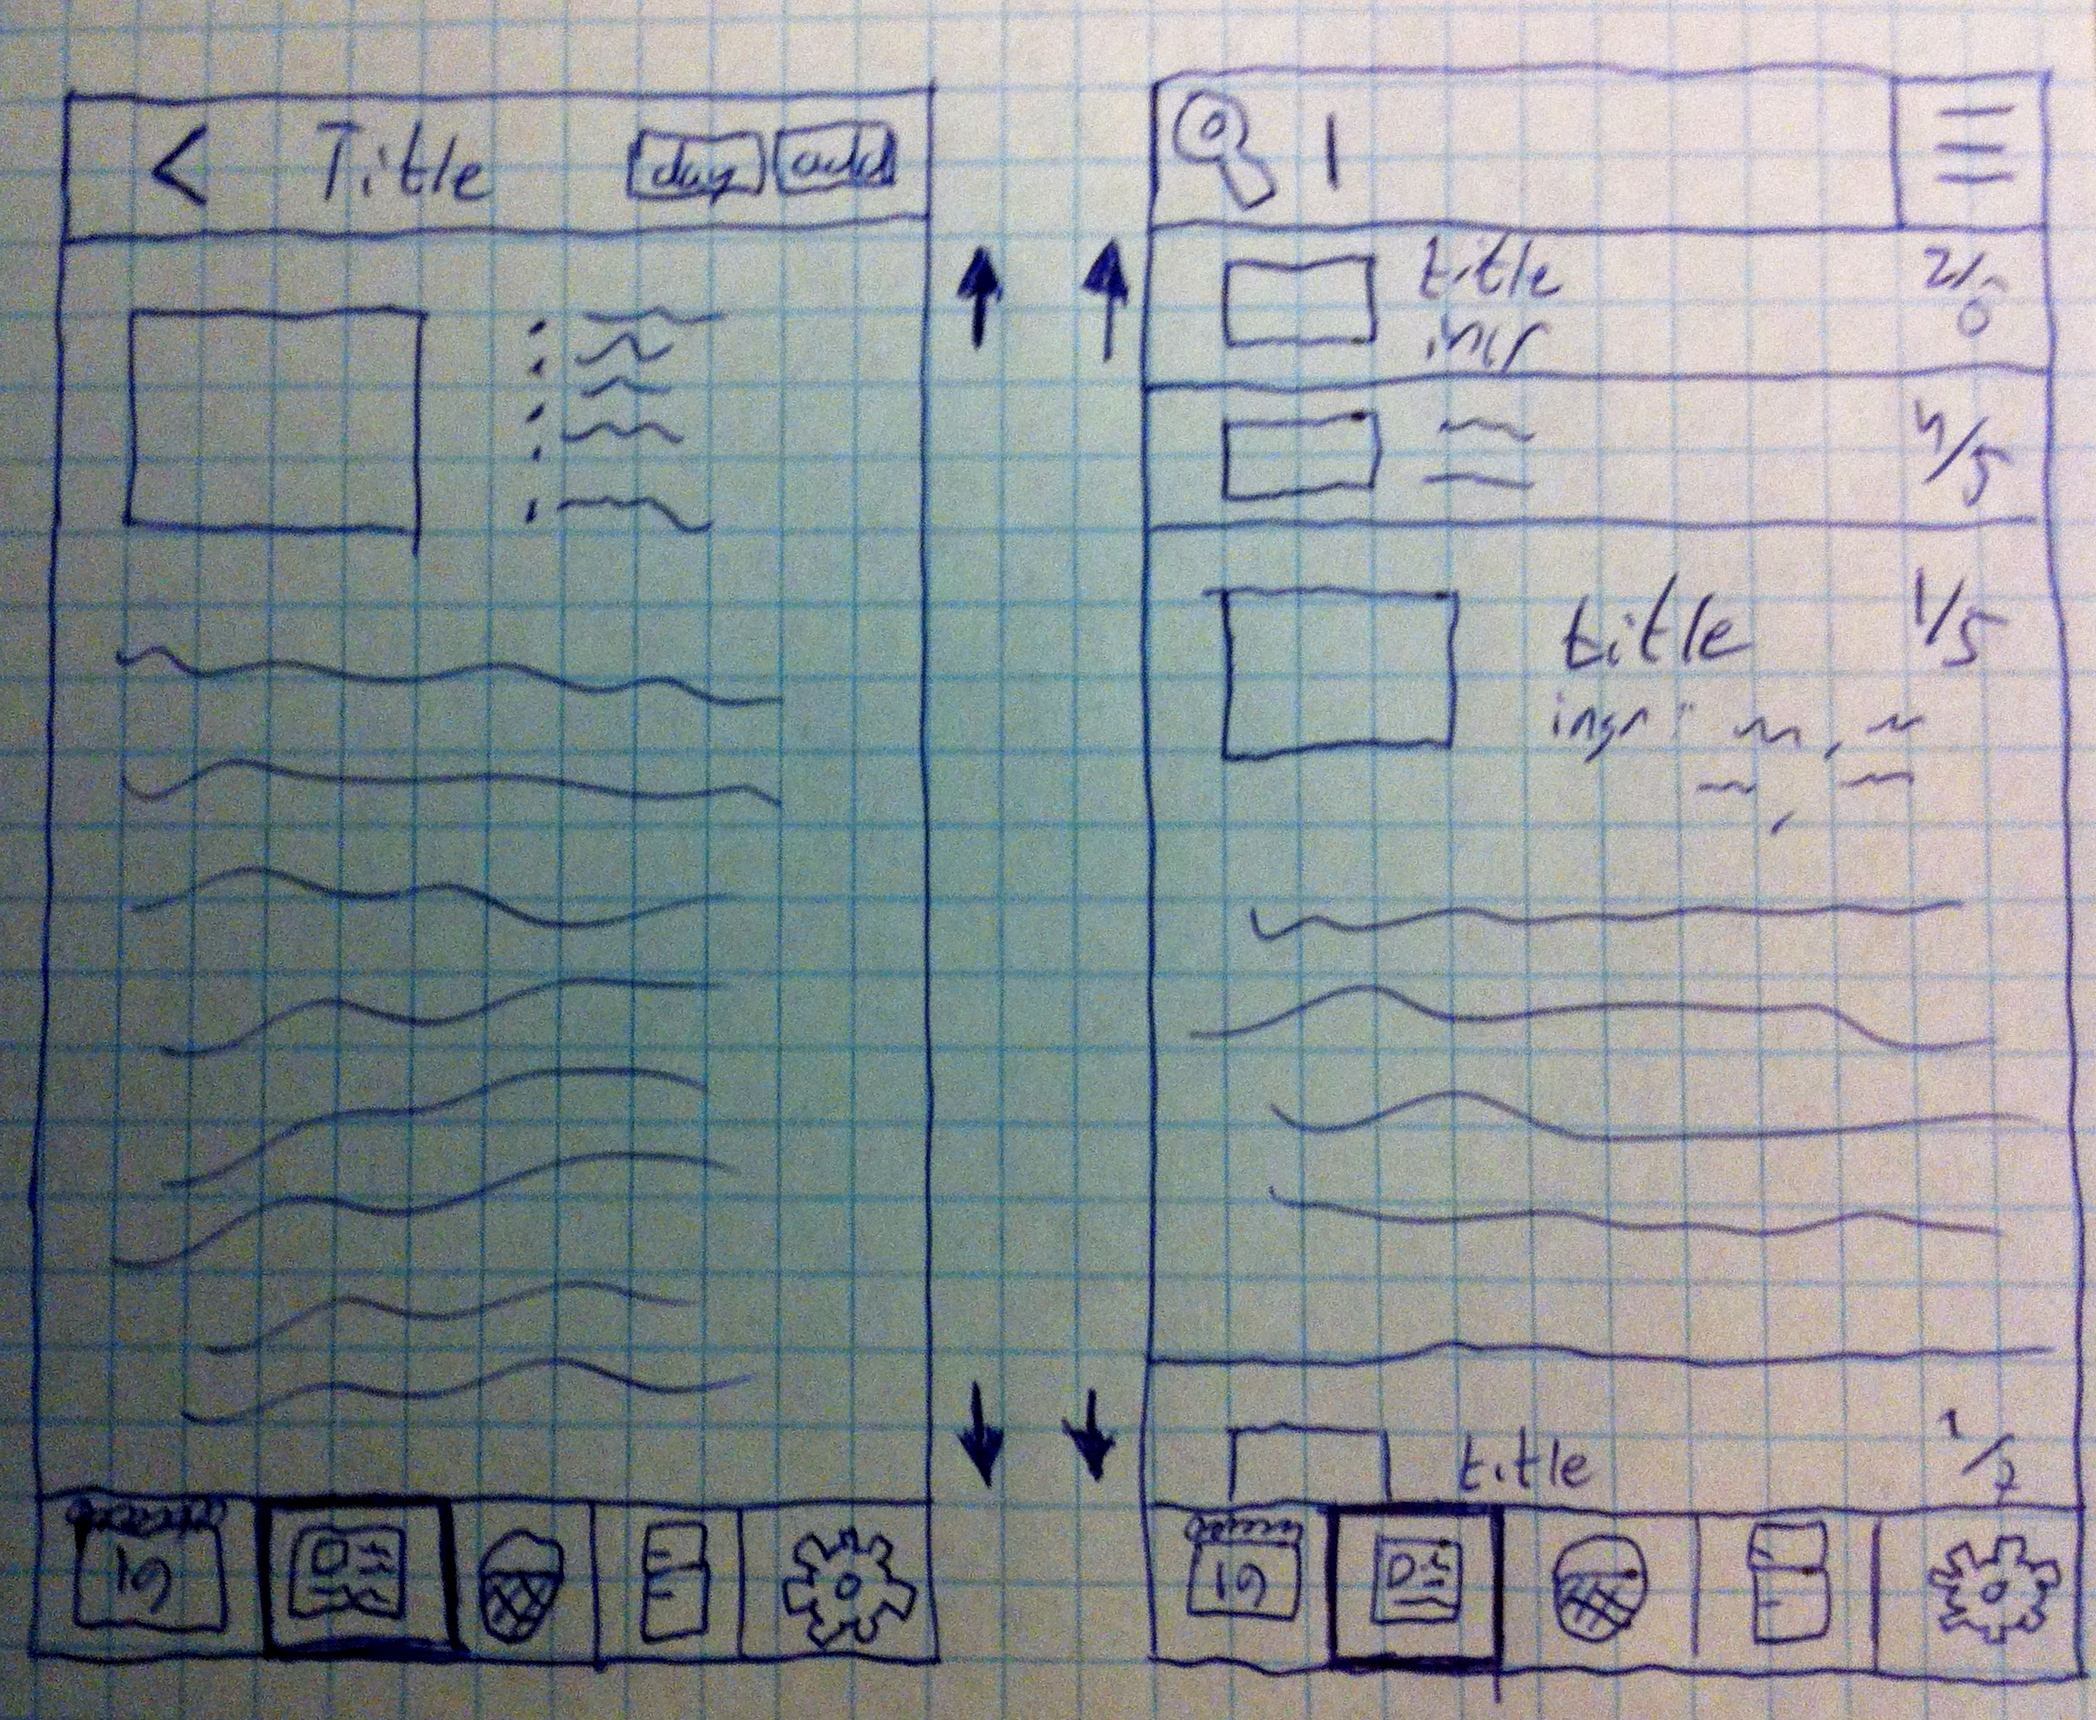
\includegraphics[width=0.5\textwidth]{Grafik/FoodPlanner/FinalRecipeBrowsingSketch2}
    \caption{One of the final sketches of the recipe browsing screen.}
    \label{FinalRecipeBrowsingSketch2}
\end{figure}

\textbf{Two screen idea:} Looking at the recipe browsing screen (right sketch on \cref{FinalRecipeBrowsingSketch2}) there are three elements to explain: 

\begin{itemize}
    \item Search bar
    \item Sort button
    \item List of recipes
\end{itemize}

The search bar is located on the top of the screen, as it is where the user is most likely to look for it at first, since this is where most search bars in mobile applications, but also websites, is located. When text is entered into the search bar, the recipes containing the text will be shown in the list of recipes. 

The sort button offers the user the functionality of sorting the list of recipes by different requirements. It might be by time to cook, by number of ingredients the user already has in the inventory, or by something else. The sort button is located at the right side of the search bar, as this was a convenient place to position it. It only consists of an icon showing that you will be able to sort the recipes by clicking the button.

The list of recipes show the recipes that the user can choose from. These are sorted by the sort button, or the search bar previously described. If there are more recipes available than the screen can display, the user will be able to swipe in an upwards motion for more recipes to appear at the bottom and the recipes at the top will disappear. In the right side of each recipe it is shown how many of the ingredients needed to make the recipe the user already have; an example is if the user has 4 out of the 10 ingredients needed the right side will show "4/10".

Looking at the specific recipe screen (left sketch on \cref{FinalRecipeBrowsingSketch2}) there are two elements to explain:

\begin{itemize}
\item Top navigation bar
\item Recipe viewing area
\end{itemize} 

The expanded recipe screen can be seen in \cref{FinalRecipeBrowsingSketch2} on the right. It is similar to the recipe browsing screen, but this screen shows more information about a specific recipe.

When the user has chosen a recipe, the user will be able to click it. By doing so, the recipe will expand, and more information about the recipe will be shown. This will only be the most relevant information, such as ingredients, cooking time, and a picture.

\begin{figure}[H]
    \centering
    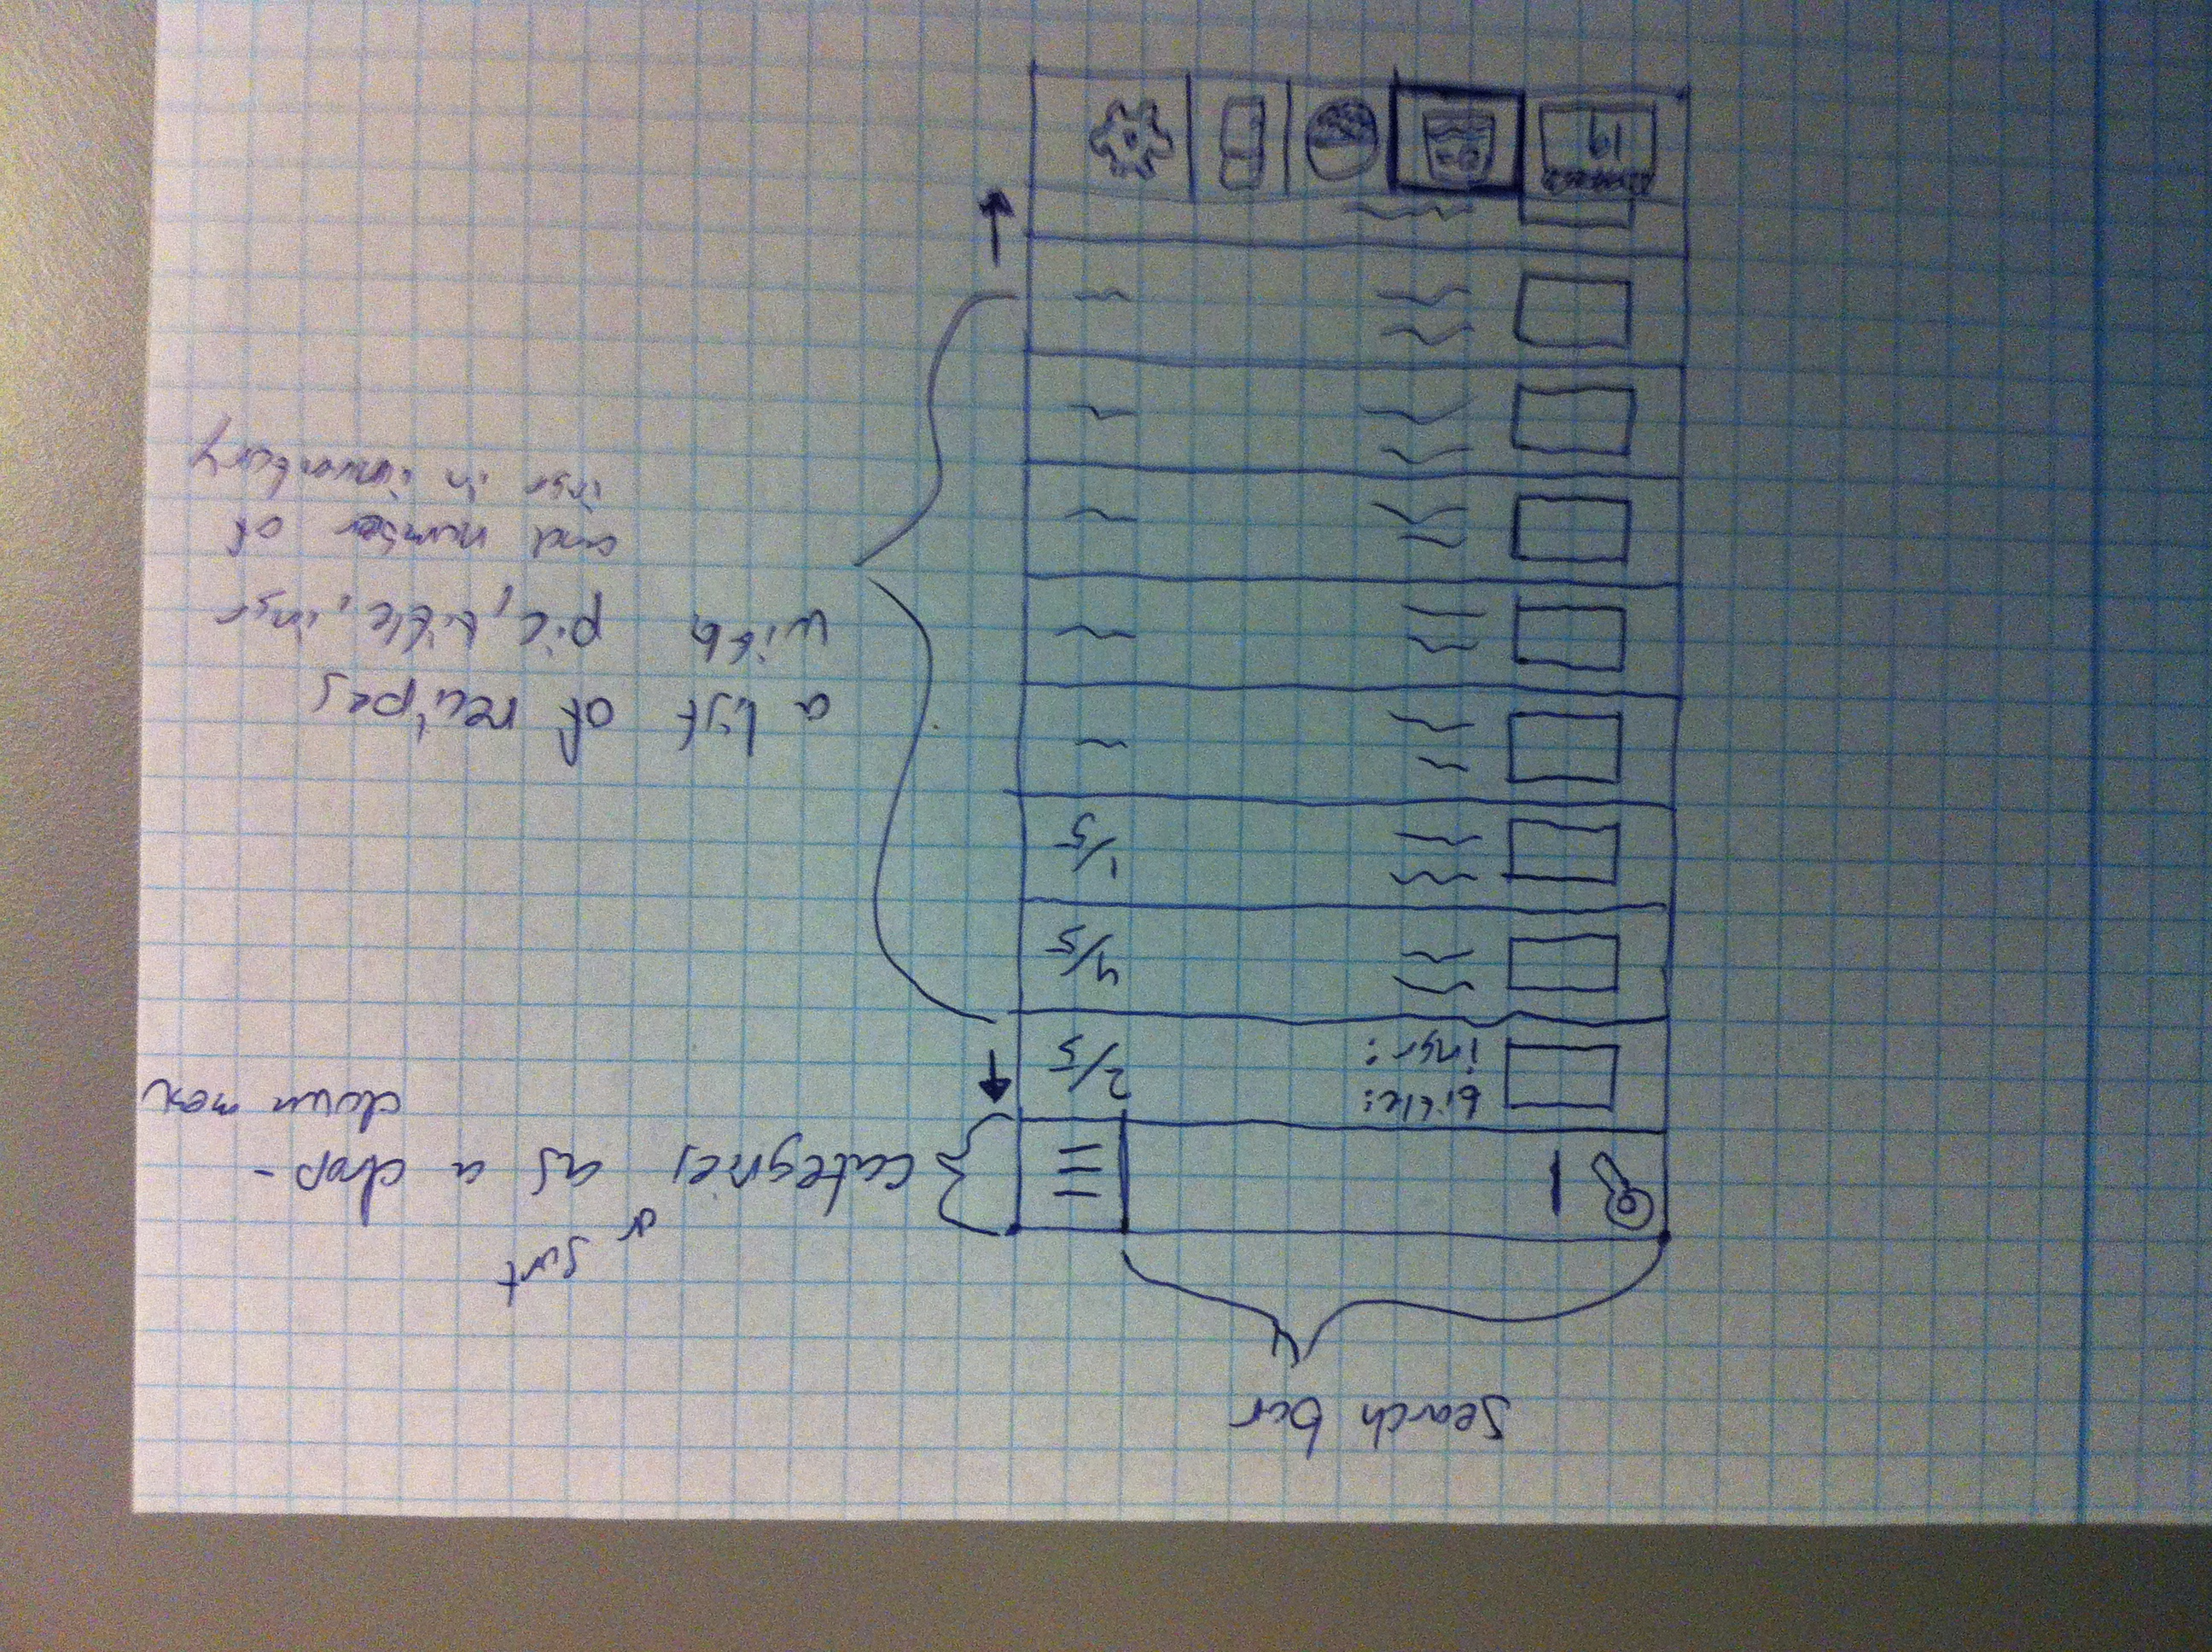
\includegraphics[width=0.5\textwidth]{Grafik/FoodPlanner/FinalRecipeBrowsingSketch1}
    \caption{One of the final sketches of the recipe browsing screen.}
    \label{FinalRecipeBrowsingSketch1}
\end{figure}

\textbf{Full screen recipe screen:} The full screen recipe screen is the left sketch on \cref{FinalRecipeBrowsingSketch2}. This screen gives the full overview of the recipe.

On the left side, a picture of the recipe will be shown if available, and the ingredients will be listed on the right side of the picture. Beneath the ingredient list, instructions on how to prepare the meal are shown. If the recipe is longer than the amount of text the screen can hold, the user will be able to scroll through the rest of the recipe by swiping.

In the top of the screen there is a navigation bar. This navigation bar gives the user the ability to do three things:

\begin{itemize}
    \item Go back
    \item Change the amount of people attending the meal
    \item Add the recipe to the meal plan
\end{itemize}

The arrow in the left of the navigation screen indicates a go back function, giving the user the ability to go back to the recipe browsing screen, if the user did not want to do anything further with the shown recipe.

The second element enables the user to change the amount of people attending the meal. This would change the amount of ingredients needed in the recipe, and would also update the shopping list, so the user would buy the right amount of the ingredients needed.

The last button gives the user functionality to add the recipe, being viewed, to the meal plan. This would update the shopping list, and add the meal to a specific day chosen by the user.
\subsection{Inventory} \label{InventoryScreen}

In this section the sketch of the inventory screen is going to be described. The functionality is going to be described as well as the design principles used in the design process. The sketch consists of 3 sketches of the screen, describing 3 different states of the inventory screen as can be seen in figure \ref{FinalInventorySketch}. The first screen from the left, shows the screen when no action has been taken. The second screen from the left shows an expanded ingredient. The third screen from the left shows the screen when the user is searching for an ingredient.

\begin{figure}[H]
    \centering
    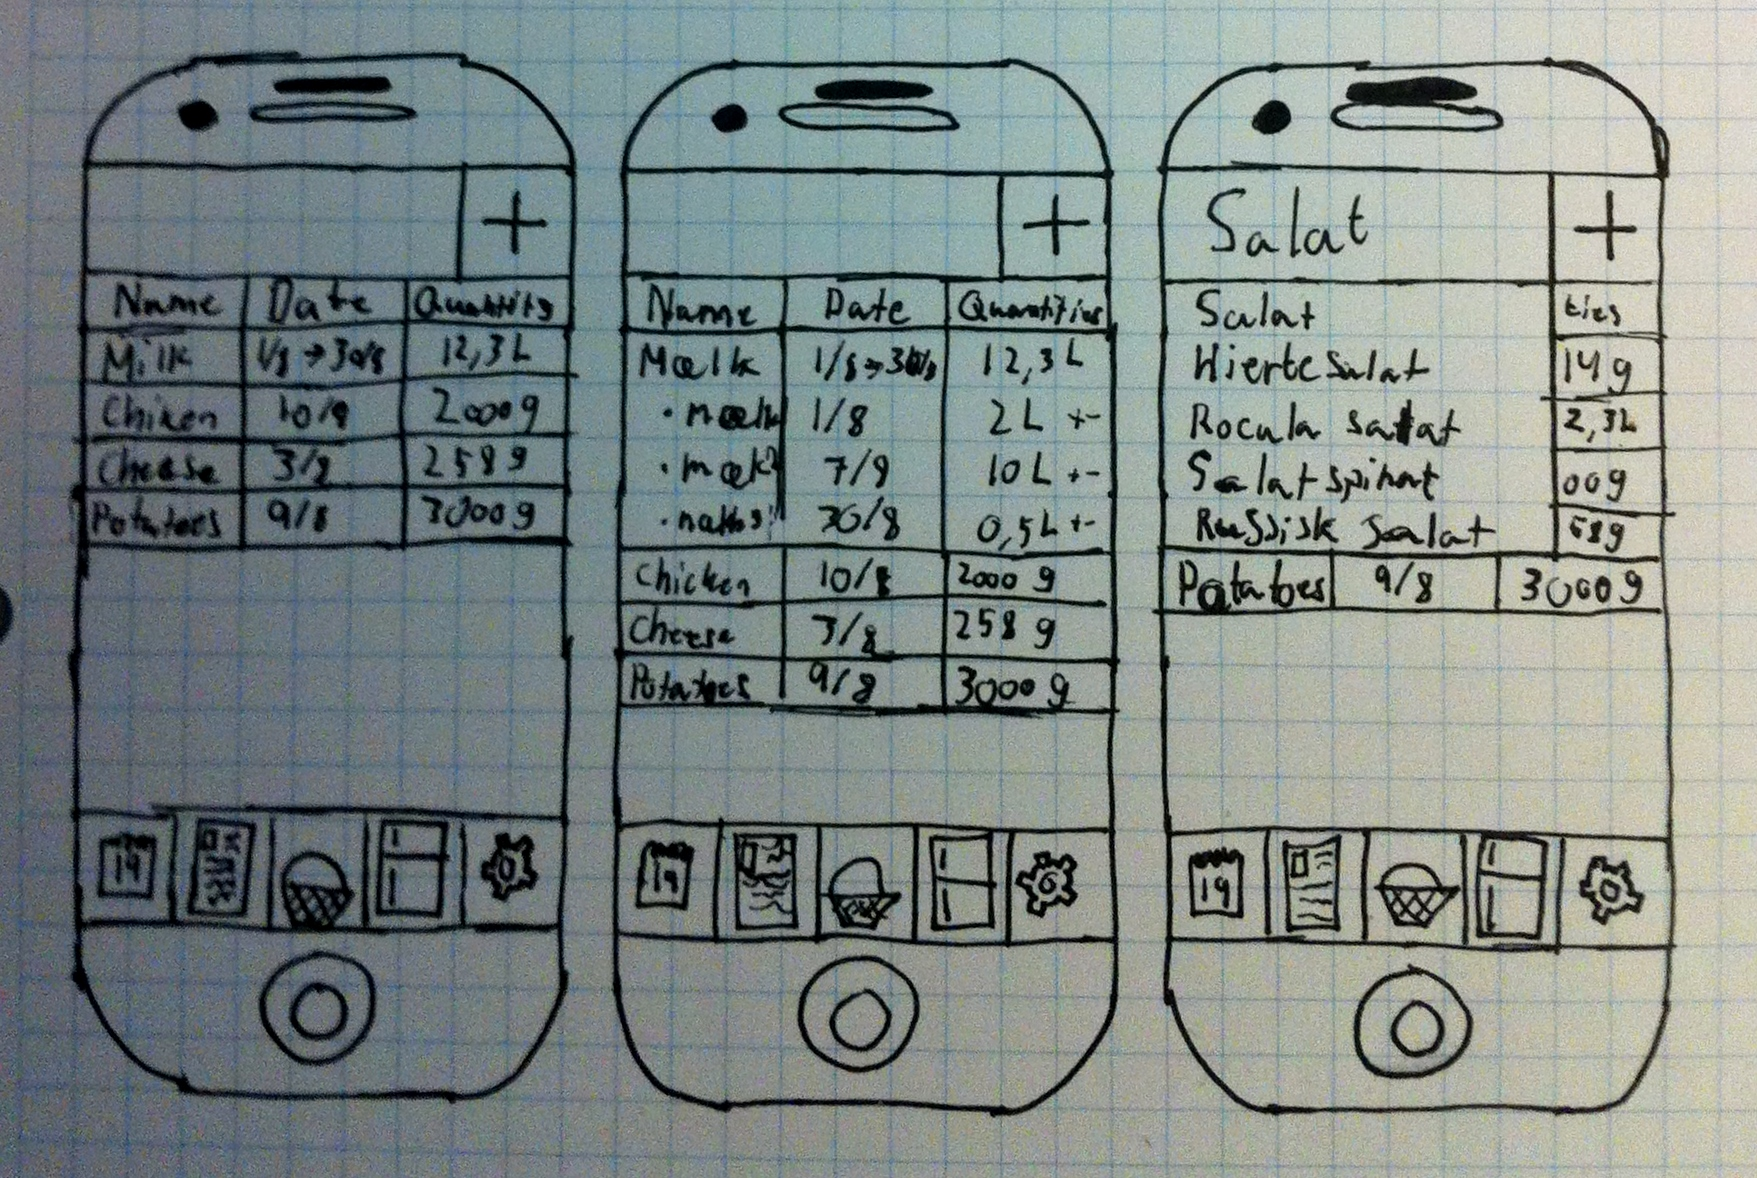
\includegraphics[width=0.5\textwidth]{Grafik/FoodPlanner/FinalInventorySketch}
    \caption{The final sketch of the inventory screens}
    \label{FinalInventorySketch}
\end{figure}

\subsection{Inventory overview screen}

The inventory overview screen is divided into two different elements, not taking the general design elements into consideration. These elements are:

\begin{itemize}
    \item Search bar
    \item Table
\end{itemize}

The search bar is placed in the top of the screen, as this is where a user most likely will look for it first, because on most mobile applications and also on websites, the search bar is located at the
top of the screen. The add icon is used to make the user able to add items to the inventory, that are not included in the ingredients of the meal plan.

The second element is the table, which is located under the search bar. The table is divided into three columns; name of the item, expiration date of the item, and the quantity of the item.

The first column with the name of the item only holds the information about the items name. The second column shows the expiration date of the item, if the user only have one instance of the item, meaning that there will only be one expiration date, only one expiration date is shown in the expiration date column, but if the user has more instances of an item and therefore different expirations dates, the first and the last expiration dates of the item will be shown, and an arrow in between the dates will indicate that the expiration dates go from the first to the last. The quantity column holds the information about the quantity of the item.

\subsection{Expanded ingredient list}

When the user click on an ingredient, the ingredient will expand and show all the instances of the information as shown on the second screen from the left in figure \ref{FinalInventorySketch}. The information is still stored in the three columns described in the inventory overview screen. An instance of the ingredient will therefore show the name of the instance, the expiration date and the quantity of the instance. 

\subsection{Searching for an ingredient}

The third screen from the left in figure \ref{FinalInventorySketch} shows the search function of the screen. When text is entered into the search box, the items in the search function will expand and lay over the ingredients in the inventory.

The search new overlay will show a fixed number of ingredients which has the searched text in their names, and the user can by clicking one of the ingredients, the expanded search bar will contract, and the item chosen will be shown in the search bar. By clicking the add icon the user will now be able to add the item to their inventory, and if the item already is in the inventory, the item will be an instance that the user can expand to see. The expiration date will then be changed in the table, as well with the quantity.
\subsubsection{Shopping list}

In this section the sketch of the shopping list is going to be described. The sketch is made up of two different screens, as seen in figure \ref{FinalShoppingListSketch}. One of the screens indicate the overview of the items on the shopping list, and the other screen shows the screen when something has been typed into the search bar.

\begin{figure}[H]
    \centering
    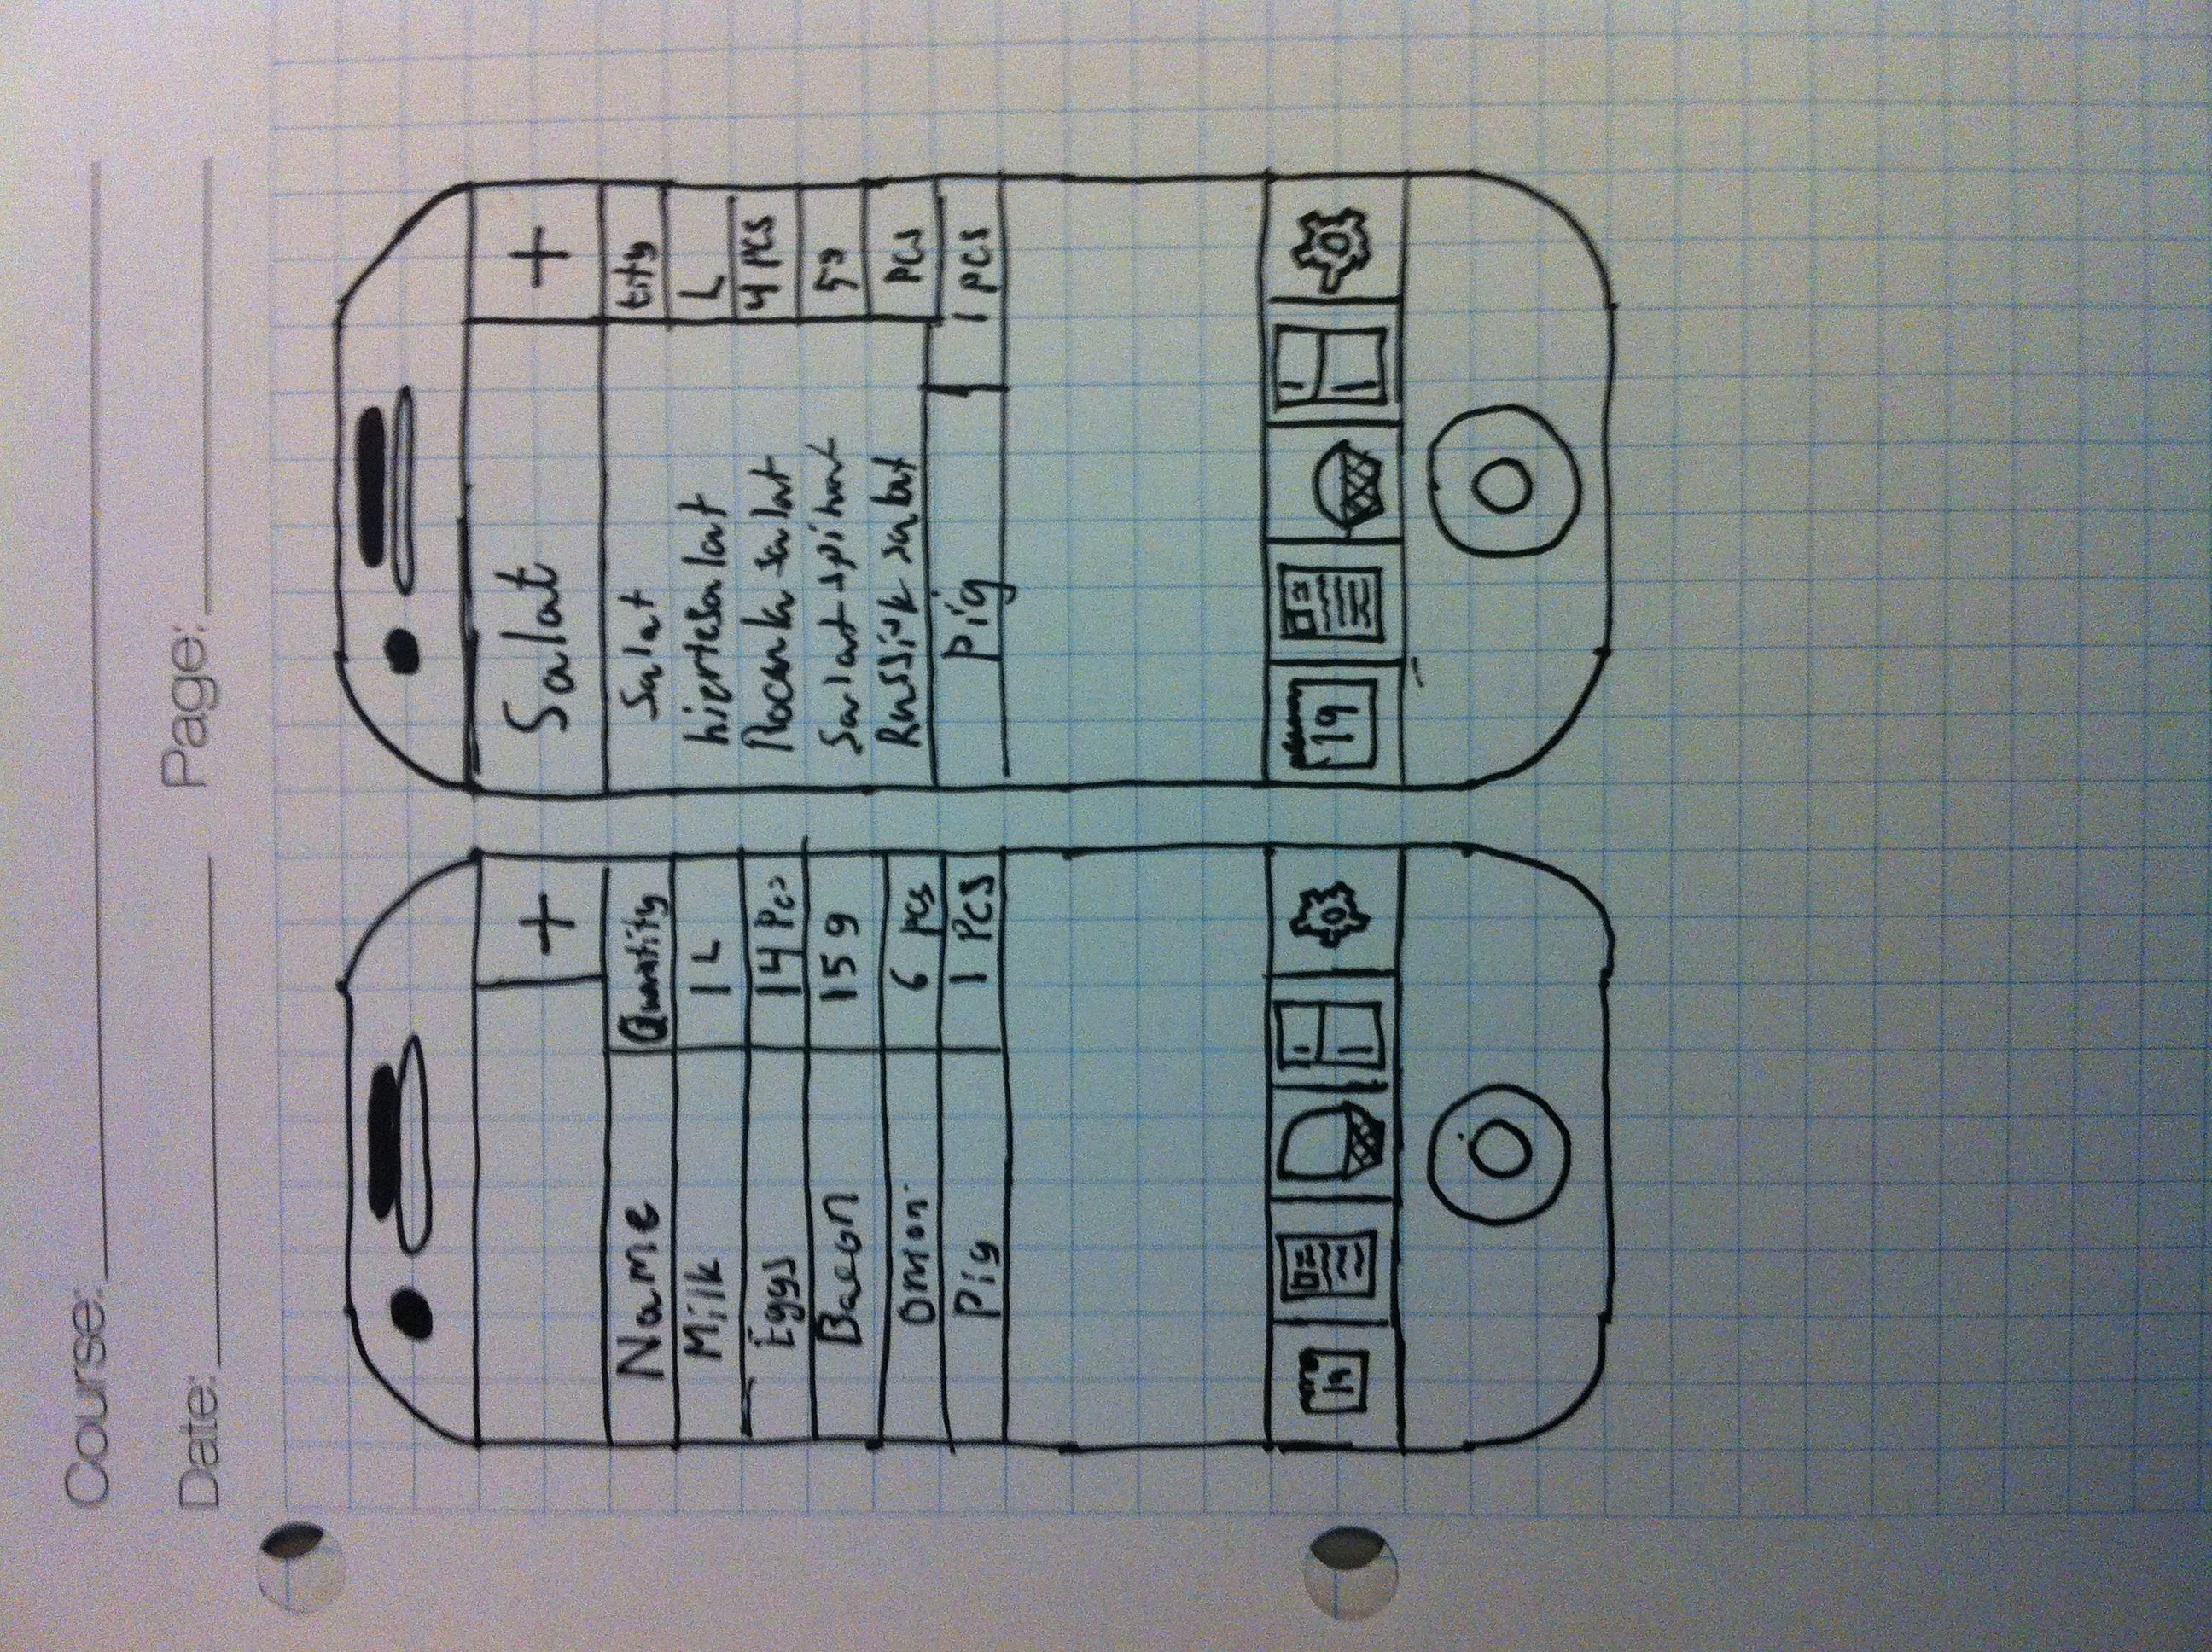
\includegraphics[width=0.5\textwidth]{Grafik/FoodPlanner/FinalShoppingListSketch}
    \caption{The final sketch of the shopping list screens}
    \label{FinalShoppingListSketch}
\end{figure}

\paragraph{Shopping List Overview screen}

The left screen in figure \ref{FinalShoppingListSketch} is the overview of the shopping list. This screen consists of two elements, not counting the general program elements, the elements is:

\begin{itemize}
	\item Search bar
	\item Table
\end{itemize}

The search bar is placed in the top of the screen, as this is where a user most likely will look for it first, because on most mobile applications and also on websites, the search bar is located at the top of the screen. The add icon is used to make the user able to add items to the inventory, that are not included in the ingredients of the meal plan.

The second element of this screen is the table, which is divided into two columns, one showing the item name, and one showing the quantity of the item. The column showing the name is broader, as the name of some items will be larger than the space needed to write the quantity.

The rows of this screens shows the ingredients on the shopping list, in the sketch, five ingredients is on the shopping list, though there could be as many as needed. If the number of different ingredients fills more than the screen can hold, the user would be able to scroll through the list by swiping upwards. Even though the user would wipe through the ingredients, the first row containing the text "Name" and "Quantity", would still be the first row.

\paragraph{Shopping List Searching Screen}

The second sketch (right sketch on \ref{FinalShoppingListSketch})  is showing the screen, when a search is performed. The screen will not change, but the search bar will expand and lay over the rest of the screen.

When a search is performed it will show a number of ingredients, in the sketch it is five, and all ingredients containing the word that have been searched for will be shown. Then the user will need to choose the ingredient they want to add to the shopping list, and click on the plus icon to add it to the list.

When a new item is added, it the user will need to go down to the quantity field, and put in the quantity of the item that will be needed.
\subsubsection{Settings}

The settings sketch can be seen in \cref{SettingsScreen} and are divided into 2 sketches. The left sketch show the list of settings, and the right sketch show the list of settings, with a specific sketch expanded.

\begin{figure}[H]
	\centering
    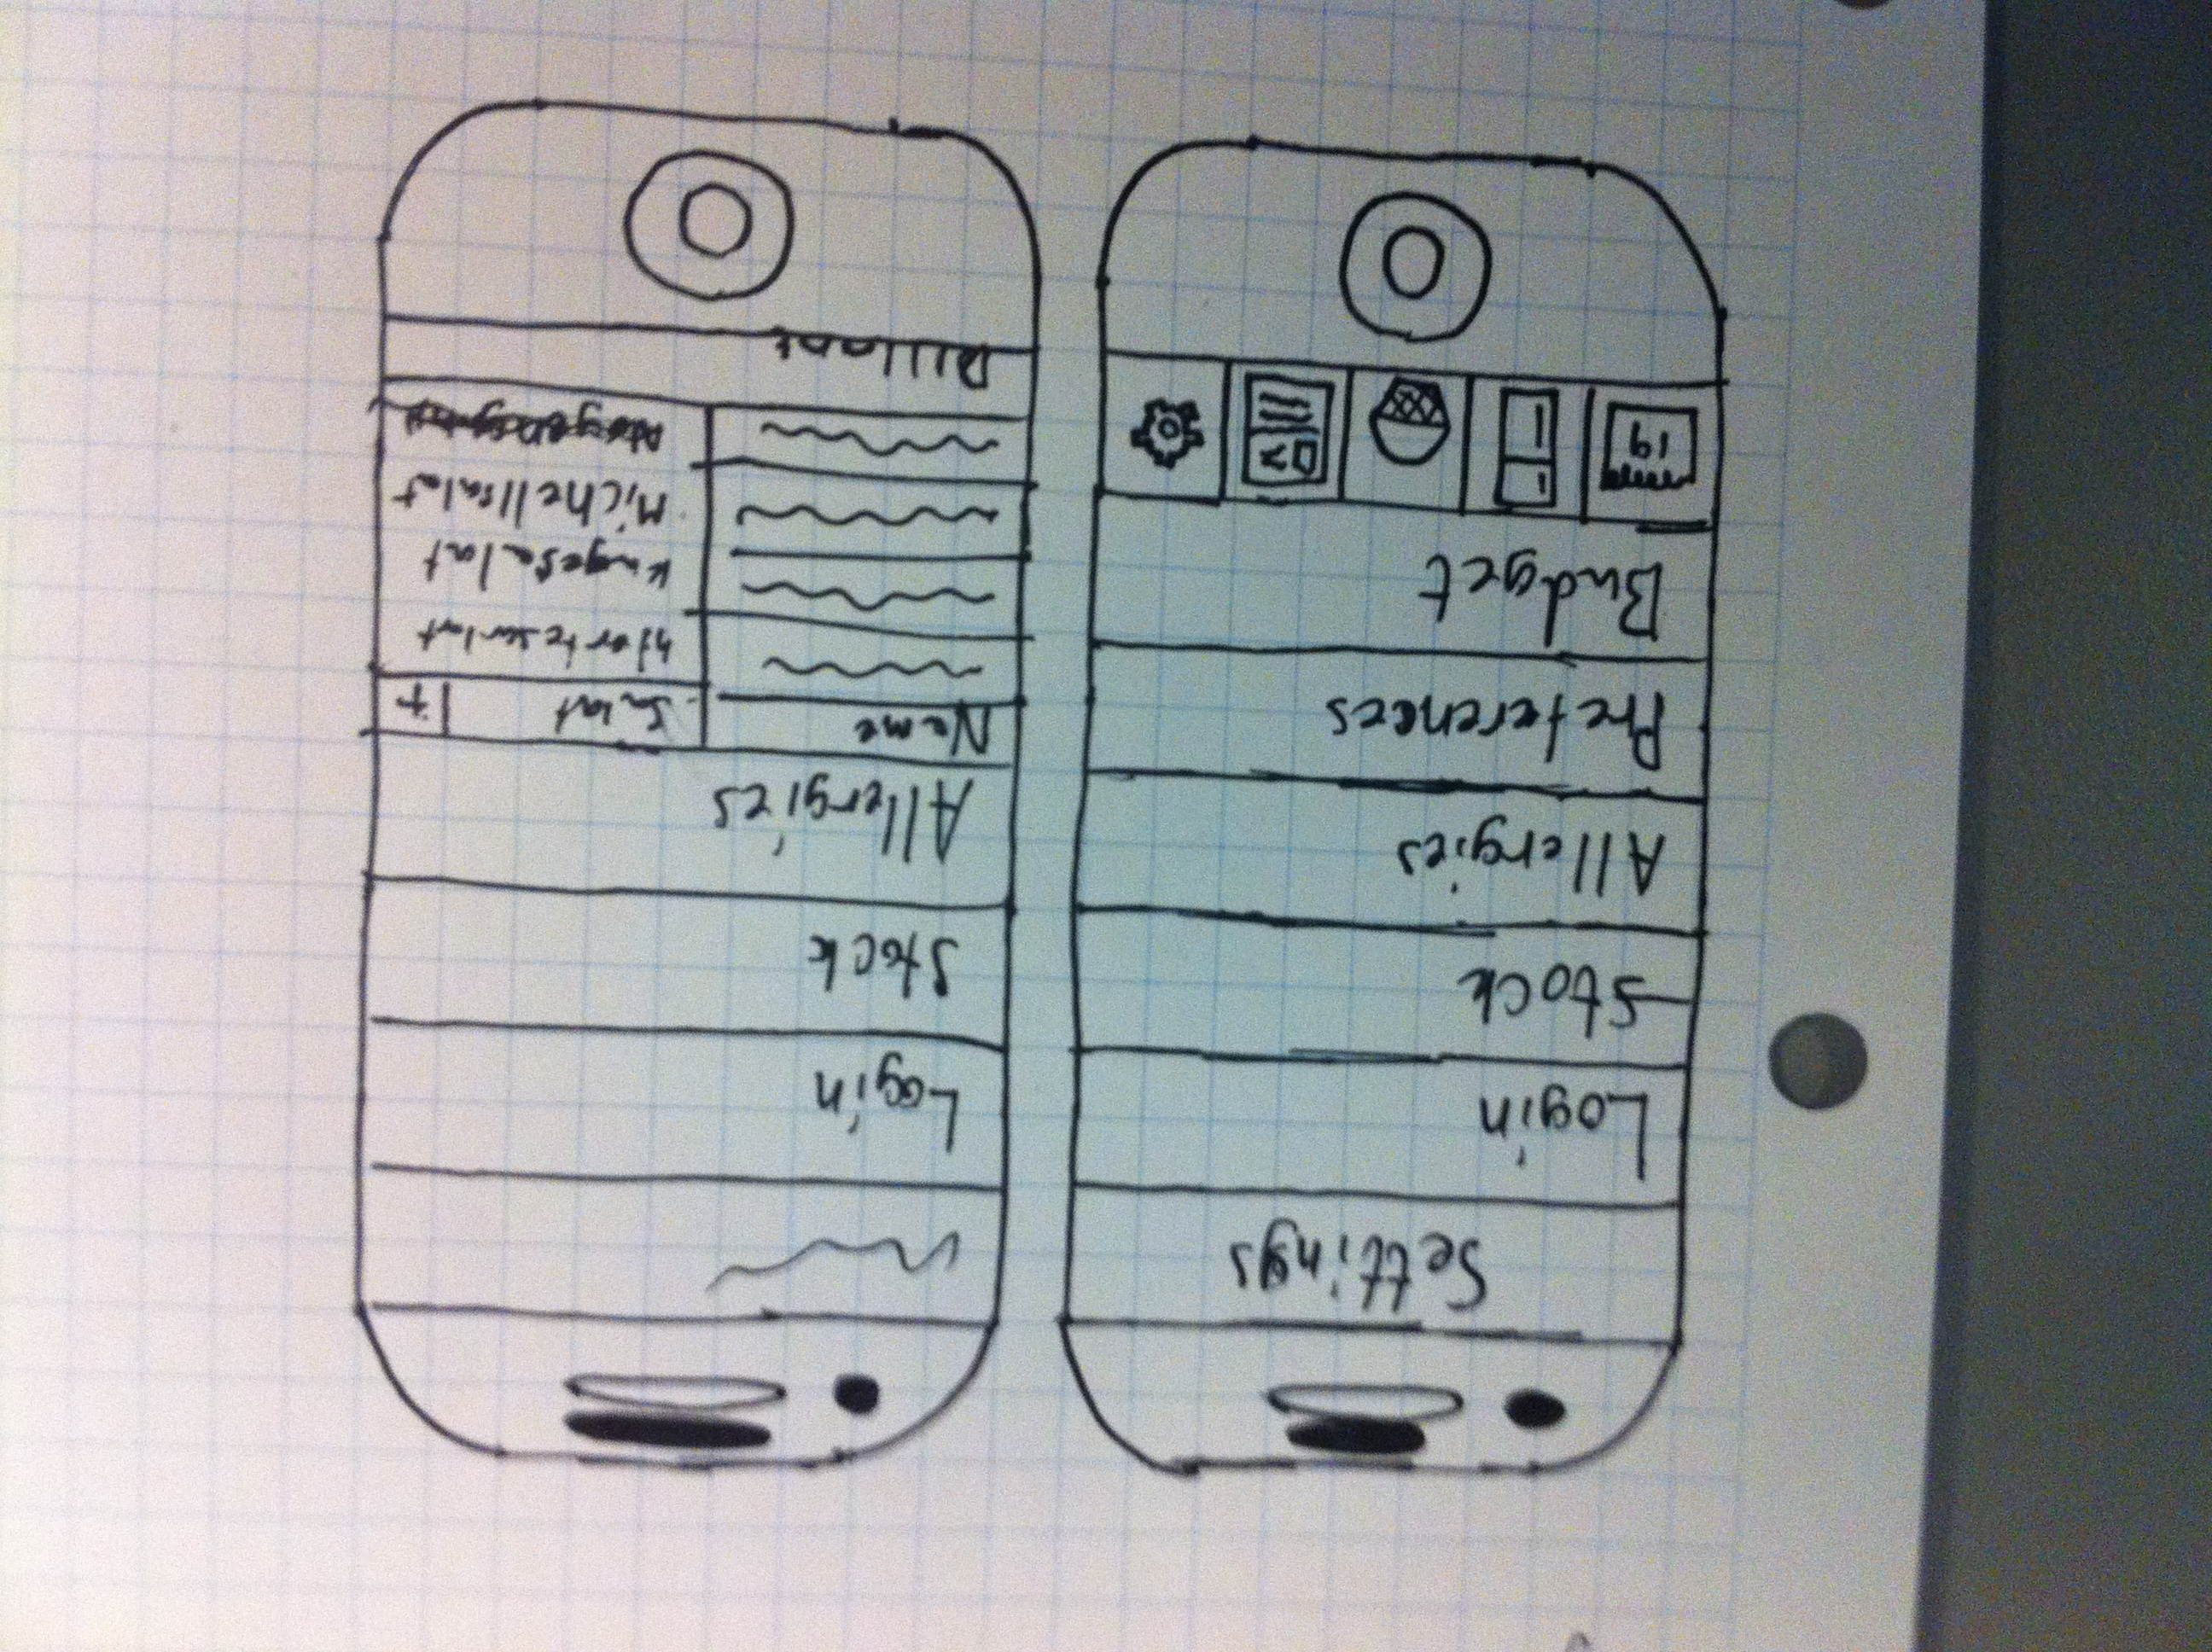
\includegraphics[width=0.5\textwidth]{Grafik/FoodPlanner/FinalSettingsSketch}
	\caption{This screen displays all of the settings in the program.}
	\label{SettingsScreen}
\end{figure}

\paragraph{Settings List} \label{SettingsList}

The setting list is the left sketch in \cref{SettingsScreen} and show a list of settings. The settings can be scrolled through, by swiping up and down, if more settings are needed than the screen can hold. The items shown in the sketch are just ideas for settings, and are just used to visualize the design idea. These are not all settings that will be incorporated in the program.

\paragraph{Expanded Settings List}

The right sketch in \cref{SettingsScreen} show the list of settings, as described in \cref{SettingsList}. Furthermore, this sketch has an expanded setting. This is because if a user click a setting,  it will expand, and show more information about this setting. In the sketch, allergies is expanded.

Expanding was chosen, because it would be consistent with the rest of the program, instead of other ideas that where discussed, for example a pop up. 

\paragraph{Colour Choice}

In order to make to program more appealing, colours are used in the design. It is important that the colours give the right statement, and that they seem attractive to the user.

The colour that was discussed first, using Paletton, was a red colour. This was supposed to be the colour of headlines and such in the program. The reason for discussing red is that red indicates appetite and food\cite{color_psychology}. Red was not chosen though, as it is too strong of a colour, and this might put the user off as it can also indicate danger or alerts.

Since red was not the optimal choice of colour, orange was considered for its similarity to red. Orange has the same quality of red to encourage appetite for the user. Furthermore is orange also a cheerful colour, and it was found to be very appealing, lastly it may be used in the program without standing out too much, or give the user wrong impressions.

\begin{figure}[H]
	\centering
    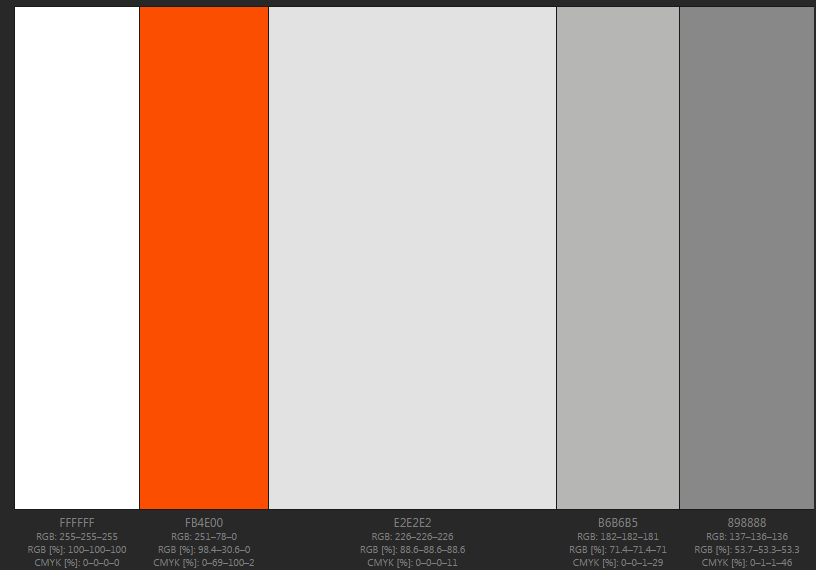
\includegraphics[width=0.9\textwidth]{Grafik/FoodPlanner/ChosenColours}
	\caption{The chosen colours for the software}
	\label{ChosenColours}
\end{figure}
\fxnote{cut some of the top of this fig. + maybe put numbers 1 to 5 on the colours, and refer to these, and not only the hashcode}
The shade of orange and a range of gray colours were chosen, and can be seen in \cref{ChosenColours}.

The colour \#898888 is used for the borders of the program. If something is parted, or a button needs a border, this colour is used. The reason for choosing this colour is that it is much darker than the other colours and gives a clear indication of an ending item.

The colour \#FB4E00 is the orange colour as can be seen in \cref{ChosenColours}. This colour is the one used for the headline text, as is the main colour of the program, since it is the only colour that can't be characterized as a neutral colour. It is only used for the headline text, as it would be difficult for the user to read the text if it was all orange.

The colour \#E2E2E2 is used for the background of the software. This is a very light colour, and it is easy to read black text on it, furthermore does the orange headlines stand more sharp, which makes them easier to see. Therefore this colour was chosen for the background. The white colour \#FFFFFF was also considered, but it was too light, and might irritate the user, lastly it did not go as well with the borders as \#E2E2E2.


    \part{Summary}

  \appendix
  \part{Appendix}
    \chapter{Interview answers}
\subsection{Interview answers}\label{Interview}
\subsubsection{25 year old single male\fxnote{What should we call these?}}
\begin{itemize}
  \item Sex: Male
  \item Age: 25
  \item Education: Vocational\fxnote{use this word for 'erhvervsuddannelse'?}
  \item Work: Skilled Sailor
  \item Household: 3 singles
\end{itemize}
\emph{What do you characterize as food waste, and is it a problem in the household?}

If any kind of food is thrown out, it is food waste according to the participant, furthermore he thinks food waste is a problem in the household, he elaborates that he thinks it is because some food is sold in bundles, that are too big compared with what is needed, and that they therefore buy too much food.

\emph{Is there a difference in the type of food, that is thrown out?}

It is mostly vegetables, which is thrown out in the household.

\emph{What factor is in focus, when food is thrown out?}

The participant only look at the freshness of the food, and does not take best before date in account.

\emph{Planning meals and shopping.}

The participant does rarely plan more than one day ahead, and does not plan at any specific time during day. Furthermore the participant mostly shop for what is wanted the specific day, and it is rarely considered, if a meal could be made from what is in the home. No one specific in the household do the shopping or the cooking, but they try to schedule the shopping with who has the time, or already has to be out.

\emph{What is the most important about your diet?}

Quality is the most important, closely followed by organic food, they try to avoid food waste, but it is not in focus.

\emph{Do you use leftovers?}

The participant always use leftovers, both because he finds it stupid, to throw it out, but also to save some money.

\emph{When do you shop, for how long, how much and how many times?}

Preferably in the morning, because there are less people. The shopping only takes 5-10 minutes and is done 4 - 5 times a week. Breakfast and lunch is often bought for a few days, where the dinner is mostly bought at the day it is needed.

\emph{What affects you in the shopping situation?}

The participant is not affected by sales in general, but do impulsive shopping if groceries are on sale, because they are close to the best before date.
\subsubsection{53 year old married female}
\begin{itemize}
  \item Sex: Female
  \item Age: 53
  \item Education: University\fxnote{use this word for 'erhvervsuddannelse'?}
  \item Work: Pedagogue
  \item Household: 2, one married couple
\end{itemize}
\emph{What do you characterize as food waste, and is it a problem in the household?}

Sales that requires you to buy to large quantities, which makes you buy to much, is seen as food waste, together with bad usage of leftovers. Food waste is not seen as a problem in this household.

\emph{Is there a difference in the type of food, that is thrown out?}

Even though food waste is not seen as a problem, it rarely happens that bread is thrown out, this is because the packages the food is sold in, are to big.

\emph{What factor is in focus, when food is thrown out?}

The participant only look at the freshness of the food, and does not take best before date in account.

\emph{Planning meals and shopping.}

The participant plan in the way that, food is taken out of the freezer in the morning, furthermore are there often made extra food, to have easy and fast prepared food, for the next few days, or to have something for a lunch, to bring to work. What needs to be shopped is mostly planned in the morning, when the food is taken out of the freezer, and the participant therefore knows what needs to be bought, if something unexpected happens, resulting in an unexpected dinner, makes shopping after work, a necessity. It is mostly the participant who does the shopping, but the other person in the household, may be asked to do some shopping.

\emph{What is the most important about your diet?}

The participant want to avoid food waste as a primary focus, next is the prize and the excitement of the meal, taken into consideration.

\emph{Do you use leftovers?}

The participant always use leftovers. And plans a dinner, so there will be leftovers, to ease the cooking for days to come.

\emph{When do you shop, for how long, how much and how many times?}

The participant prefers to shop after work. The shopping only takes about 10 minutes and is done 3-4 times a week. furthermore the participant prefers to shop for a few days only, to keep the food fresh. this results in a fridge that in quite empty, and as a result, the shopping is often a necessity.

\emph{What affects you in the shopping situation?}

The participant is affected by "decorated" sales mend for tempting to do impulsive shopping, furthermore the participant does not like to buy the food that is on sale, because it is close to the best before date.
\subsubsection{75 year old married female}
\begin{itemize}
  \item Sex: Female
  \item Age: 75
  \item Education: Vocational\fxnote{use this word for 'erhvervsuddannelse'?}
  \item Work: Pensioner
  \item Household: 2, one married couple
\end{itemize}
\emph{What do you characterize as food waste, and is it a problem in the household?}

No use of leftovers, and food that is badly stored, which makes it go bad. Food waste is not seen as a problem in the household, if there are small leftovers, the dog will get it.
%Sales that requires you to buy to large quantities, which makes you buy to much, is seen as food waste, together with bad usage of leftovers. Food waste is not seen as a problem in this household.

\emph{Is there a difference in the type of food, that is thrown out?}

The participant can not say what difference there could be, because food is never thrown out.

\emph{What factor is in focus, when food is thrown out?}

If food would be thrown out, the freshness will be the only factor.

\emph{Planning meals and shopping.}

The participant likes to shop large quantities of meat, because it is bought from a butcher who's shop is far away from home. Where items like bread and milk is bought as needed, the participant elaborates that there is rarely missing anything, because alternative ingredients will be found.

\emph{What is the most important about your diet?}

It is important that the diet if healthy, and filled with energy, the meat has to be proper, and therefor it is bought from a butcher

\emph{Do you use leftovers?}

The participant always use leftovers.

\emph{When do you shop, for how long, how much and how many times?}

There is no specific time in the day which the participant likes to shop, and the shopping takes place 2 to 3 times a week.

\emph{What affects you in the shopping situation?}

The participant likes to buy savings, and fill the freezer, and can be tempted to do impulsive shopping, furthermore the participant likes to buy the food that is on sale, because it is close to the best before date.

\subsubsection{55 year old single woman}
\begin{itemize}
  \item Sex: Female
  \item Age: 55
  \item Education: Skilled Worker\fxnote{use this word for 'faglært'?}
  \item Work: Teaching assistant
  \item Household: 2, mother and daughter
  \item Phone: Yes, android
  \item Tablet: Yes, android
\end{itemize}

\emph{What do you characterize as food waste?}

When food is thrown out in the trash. This applies to both prepared and unprepared food. If animals are fed with the food instead of it getting thrown out, it is not food waste.

\emph{Is foodwaste a problem for the household?}

No, everything edible that gets too old, it is fed to the animals of the household, more specifficaly hens, as a replacement of fodder.

\emph{Is there a difference in what gets thrown out?}

No, there is nothing specific that gets thrown out the most.

\emph{What factors are considered when throwing food out?}

Mostly the freshness of the food. Not so much the best before date, but mostly how the food looks, feels, and smells.

\emph{When do you plan your meals and shopping?}

The planning is done a 2-3 days ahead of when the food is getting eaten.

\emph{How is the shopping planned?}

Mostly out of what is wanted to eat and discounts.

\emph{How is the coordination of the members of the household?}

The mother makes everything, the daughter neither prepares the food or does any shopping.

\emph{What is valued the most about your diet?}

What the household want to eat, variation of the meals, and a little economy.

\emph{Do you use leftovers?}

Yes, leftover gets used for lunch or dinner, depending on the qunatity of the leftovers.

\emph{When do you grocery shop?}

In the morning before work, or after dinner.

\emph{How long does the grocery shopping take?}

About an hour because there is being shopped in more than one store.

\emph{How many times a week is grocery shopping done?}

3 times a week.

\emph{WHat is the quantity when shopping?}

Depends from time to time.

\emph{What affects you in the groecry shopping situation?}

The discounts are planned from home, as the participant looks through discount magzines. But if there is something practical and cheap, the particapant will buy on impulse.

\emph{How do you make your shopping list?}

The shopping list is made in by hand on a notepad, but if there was a simple solution for tablet or smartphone, the participant would be willing to try it out. The participant have already tried using Evernote for a shopping list that would sync between different devices.
\subsubsection{28 year old single male}
\begin{itemize}
  \item Sex: Male
  \item Age: 28
  \item Education: Educator
  \item Work: Kindergarten helper
  \item Household: 11
\end{itemize}
\emph{What do you characterize as food waste, and is it a problem in the household?}

The participant believes when eat able food is thrown out, is should be considered food waste. He does not feel that the food waste level in the household is a problem.

\emph{Is there a difference in the type of food, that is thrown out?}

It is mostly vegetables, which is thrown out in the household, he does not always have the time to eat them all before they goes bad.

\emph{What factor is in focus, when food is thrown out?}

When the participant feels the food has become to old he will throw it out, this is based on how fresh the food seems to be.

\emph{Planning meals and shopping.}

How the participant plans his shopping and cooking varies, but the planning happens for the most part when he already is at the mall. When he is shopping for products, his choosing is based on what he likes and what there is on sale. He is alone when he is shopping or cooking.

\emph{What is the most important about your diet?}

It can not be to spicy as he is vulnerable to stomach ulcers. It also has to be of a good quality and economic.

\emph{Do you use leftovers?}

The participant tries to save and eat leftovers when possible.

\emph{When do you shop, for how long, how much and how many times?}

He tries to do his shopping after work if possible. He is not sure about how much time he spends on shopping, but the time used goes down he know what he wants beforehand.

\emph{What affects you in the shopping situation?}

He tries to get the wares he finds delicious, or if they are on sale.
\chapter{Personas} \label{PersonasAppendix}
\section{Personas}
This part will show three different personas.

\subsection{Henrik Jensen}
\begin{figure}[H]
	
\includegraphics[width=0.30\textwidth]{Grafik/FoodPlanner/PersonaHenrikJensen}
	\label{PersonaHenrikJensen}
\end{figure}
\begin{itemize}
	\item Age: 38
	\item Relational status: Married
	\item Children: 2, age 16 and 14
	\item Occupation: Working as an IT consultant.
	\item Preferences: Wanna spend less time on shopping but still cook delicious dinners.
\end{itemize}
-Henrik drives home after he has finished a meeting with a costumer. The meeting dragged on and Henrik Just want to get home and get a nice dinner.

-His wife is working as a nurse and has a late night shift this evening. It is therefore up to Henrik to cook Dinner for the whole family

-On his way home he stops by the local supermarket and on his way to the entrance he starts to plan what he will prepare for dinner.

-He finds some meat on sale which he decides to buy.

-When he gets home he finds the recipe he wanted and starts to cook.

-It annoys him slightly that he does not plan ahead and very variated. Bu he fells he ha no other choice because of his work schedule and his desire to reduce shopping time.

-After dinner he starts the washing machine and turns on tv to watch football. He is an football enthusiast and played it himself when he was younger. 

\subsection{Peter Nielsen}
\begin{figure}[H]
	
\includegraphics[width=0.15\textwidth]{Grafik/FoodPlanner/PersonaPeterNielsen}
	\label{PersonaHenrikJensen}
\end{figure}
\begin{itemize}
	\item Age: 23
	\item Relational status: Single
	\item Children: None
	\item Occupation: Student
	\item Preferences: Does not spend more time in the kitchen than needed.
\end{itemize}
-Peter has classes till late afternoon, so when he gets of school he rushes home, and does not care about dinner when he leaves school.

-Peter first plans what he is going to have for dinner when he get home. At this point he is usually just plans something that is fast to make.

-When he has to shop he goes for the nearest shop, and just buys what the recipe says, and does not look at what is on sale.

-When he gets home after buying the ingredients, he wait till he is hungry before starting making the food.

-He is slightly annoyed that he does not plan ahead but he blames that he has no things to help him seclude his plans.

-After dinner he starts he goes sit in front of the computer where he starts playing video games with his friends.

\subsection{Anne Madsen}
\begin{figure}[H]
	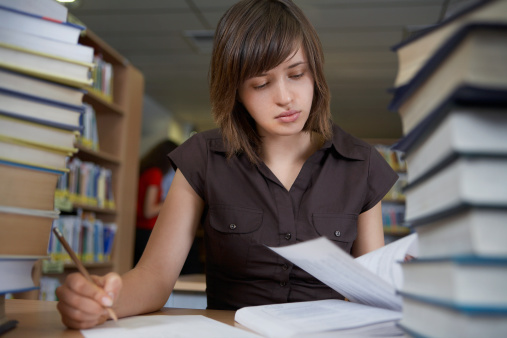
\includegraphics[width=0.25\textwidth]{Grafik/FoodPlanner/PersonaAnneMadsen}
	\label{PersonaHenrikJensen}
\end{figure}
\begin{itemize}
	\item Age: 18
	\item Relational status: Single
	\item Children: None
	\item Occupation: Student
	\item Preferences: Likes to spend time in the kitchen to prepare a good fresh meal with vegetables
\end{itemize}
-Anne has classes till late afternoon, after school Anne has a specific shopping list based on what she has to buy to make food for dinner.

-Anne does not know where to find the cheapest groceries which she finds slightly annoying, so she keeps shopping the same place as she has always done.

-When Anne is done shopping she decides that it is too dangerous to ride her bike with a bag of groceries hanging of her handlebar. So she decides to pull her bike home.

-When Anne finally gets home the trip from school to home has taken so long that it is time to make dinner.

-After dinner she cleans the plates, and gets ready to prepare her homework for the next day. 

\chapter{Usability Test Tasks}
\subsection{Usability Test Tasks} \label{UsabilityAppendix}

When the test subjects of the usability test had been told how the test was conducted, they where given a list of taks that they had to perform within the program, to test the usability. These tasks are described underneath.

\textbf{Task 1}
You have nothing planned for tonight's meal, and you feel like having \textit{chicken and leek pie}.
\begin{itemize}
    \item Search for and add the \textit{chicken and leek pie} recipe for today’s meal
\end{itemize}

\textbf{Task 2}
On the way home from work, you want to do some shopping for tonight’s meal, but because you are on a bike, you cannot shop many items; therefore you want to change the number of days to shop for.
\begin{itemize}
    \item Navigate to the page that allows you to change number of days to shop for, and change this to 1.
\end{itemize}

\textbf{Task 3}
You have been doing some shopping for tonight’s \textit{chicken and leek pie} and want to add some bought items to your inventory
\begin{itemize}
    \item Find \textit{onion}, \textit{egg} and \textit{leek} on the shopping list and add them to the inventory list.
\end{itemize}

\textbf{Task 4}
You had a dinner planned with some friends, but due to bad planning from your friends, you have to cancel your plans.
\begin{itemize}
    \item Go to week 51, and remove \textit{Spinach and Cheese Souffle} from Monday the 15th of December.
\end{itemize}

\textbf{Task 5}
During the last shopping trip you also bought 5 \textit{lollipop sticks}. These have an expiration date that says \textit{16th of July 2017}.
\begin{itemize}
    \item Add 5 \text{lollipop sticks} to the inventory and change their expiration date to \textit{16th of July 2017}
\end{itemize}

\textbf{Task 6}
Friends have invited you over for a party Sunday the \textit{14th of December}, so you have to reschedule the meal you have planned for this day
\begin{itemize}
    \item Change the date of the meal on the \textit{14th of December} to be scheduled for a week later.
\end{itemize}

\textbf{Task 7}
After a long day, you feel like being good to yourself, you therefore eat some of the \textit{white chocolate} you have.
\begin{itemize}
    \item Remove \textit{100 ml} of \textit{white chocolate} from the inventory
\end{itemize}

\textbf{Task 8}
You have some friends over, when you decide to have some \textit{beer}
\begin{itemize}
    \item Remove all \textit{beer} from the inventory
\end{itemize}

\textbf{Task 9}
It is Christmas and you feel like having something with \textit{cinnamon} in it.
\begin{itemize}
    \item Search for recipes with \textit{cinnamon} and add one for today.
\end{itemize}

\textbf{Task 10}
You are having friends over for dinner \textit{Friday the 19th of December}; you know that you will be 9 persons in total
\begin{itemize}
    \item Find the recipe \textit{Hot and Smoky Cheeseburgers with Bacon and Pickled Cherry Pepper Relish} and add it for the \textit{19th of December}
    \item Change the number of meal participants to 9
\end{itemize}

\textbf{Task 11}
Because it is Christmas you decide that you want more recipes with \textit{cinnamon} to be shown.
\begin{itemize}
    \item Add \textit{cinnamon} to the list of rated ingredients with a rating of 100
\end{itemize}

\subsubsection{Follow-up questions}

After a test had been conducted, some follow-up questions were asked to find if the test participants had any comments about the usability of the program.

\begin{itemize}
    \item Do you have any general comments about the program?
    \item Did you find the program easy to use?
    \item Was the text easy to read, even though some of it were orange, and the background where grey?
    \item Did it make sense that the functionalities in the settings screen where placed there, or should they have been placed in other pages?
    \item Did the rate ingredients function make sense? Was 100 too many? Would 10 stars have been better?
    \item How did navigation work through the program? Was it easy to navigate through pages?
\end{itemize}
    \printbibliography
    
    % list of fxnotes that needs to be fixed
    \listoffixmes

\end{document}